% Created 2020-02-12 Wed 10:25
% Intended LaTeX compiler: pdflatex
\documentclass[11pt]{article}
\usepackage[utf8]{inputenc}
\usepackage[T1]{fontenc}
\usepackage{graphicx}
\usepackage{grffile}
\usepackage{longtable}
\usepackage{wrapfig}
\usepackage{rotating}
\usepackage[normalem]{ulem}
\usepackage{amsmath}
\usepackage{textcomp}
\usepackage{amssymb}
\usepackage{capt-of}
\usepackage{hyperref}
\usepackage{minted}
\usepackage{/home/ryan/Dropbox/profiles/Templates/LaTeX/ScreenStyle}
\author{Ryan G}
\date{\today}
\title{Introduction to Data Science}
\hypersetup{
 pdfauthor={Ryan G},
 pdftitle={Introduction to Data Science},
 pdfkeywords={},
 pdfsubject={},
 pdfcreator={Emacs 28.0.50 (Org mode 9.3.4)}, 
 pdflang={English}}
\begin{document}

\maketitle
\tableofcontents

\section{Simple Linear Regression\hfill{}\textsc{IntroDataSci}}
\label{sec:orgad9bff5}
Material of Tue 12 2019, week 2
\subsection{Load Packages}
\label{sec:orge805c55}
\begin{minted}[]{r}
# Load Packages
if(require('pacman')){
  library('pacman')
}else{
  install.packages('pacman')
  library('pacman')
}

pacman::p_load(caret, scales, ggplot2, rmarkdown, shiny, ISLR, class, BiocManager,
               corrplot, plotly, tidyverse, latex2exp, stringr, reshape2, cowplot, ggpubr,
               rstudioapi, wesanderson, RColorBrewer, colorspace, gridExtra, grid, car,
               boot, colourpicker, tree, ggtree, mise, rpart, rpart.plot, knitr, MASS,
               magrittr, EnvStats,tidyverse,tidyr,devtools, bookdown, leaps, car, clipr,
               tikzDevice, e1071)



mise()
set.seed(0932)
\end{minted}

\subsection{Question 1}
\label{sec:org058c0ed}
\subsubsection{(a) Import the Data\hfill{}\textsc{ATTACH}}
\label{sec:org7a71359}
\begin{minted}[]{r}
setwd("/home/ryan/Dropbox/Notes/DataSci/IntroDataSci/Org-Babel/")
getwd()
adv <- read.csv(file = "../../data/83/4c42c3-8dd8-4fef-b402-7e341764d5e9/Advertising.csv", header = TRUE, sep = ",")
\end{minted}

\begin{enumerate}
\item Inspect the structure of the Data Set
\label{sec:orgd878f52}
\begin{minted}[]{r}
head(adv)
\end{minted}

\begin{verbatim}
   ##      TV Radio Newspaper Sales
   ## 1 230.1  37.8      69.2  22.1
   ## 2  44.5  39.3      45.1  10.4
   ## 3  17.2  45.9      69.3   9.3
   ## 4 151.5  41.3      58.5  18.5
   ## 5 180.8  10.8      58.4  12.9
   ## 6   8.7  48.9      75.0   7.2
outputoutputoutput
 #valuevaluevalue+Bboth boutput 
 str(adv)
 #+END_SRC

 #+BEGIN_EXAMPLE
   ## 'data.frame':    200 obs. of  4 variables:
   ##  $ TV       : num  230.1 44.5 17.2 151.5 180.8 ...
   ##  $ Radio    : num  37.8 39.3 45.9 41.3 10.8 48.9 32.8 19.6 2.1 2.6 ...
   ##  $ Newspaper: num  69.2 45.1 69.3 58.5 58.4 75 23.5 11.6 1 21.2 ...
   ##  $ Sales    : num  22.1 10.4 9.3 18.5 12.9 7.2 11.8 13.2 4.8 10.6 ...
\end{verbatim}

\begin{minted}[]{r}
summary(adv)
\end{minted}

\begin{verbatim}
##        TV             Radio          Newspaper          Sales
##  Min.   :  0.70   Min.   : 0.000   Min.   :  0.30   Min.   : 1.60
##  1st Qu.: 74.38   1st Qu.: 9.975   1st Qu.: 12.75   1st Qu.:10.38
##  Median :149.75   Median :22.900   Median : 25.75   Median :12.90
##  Mean   :147.04   Mean   :23.264   Mean   : 30.55   Mean   :14.02
##  3rd Qu.:218.82   3rd Qu.:36.525   3rd Qu.: 45.10   3rd Qu.:17.40
##  Max.   :296.40   Max.   :49.600   Max.   :114.00   Max.   :27.00
\end{verbatim}
\end{enumerate}
\subsubsection{(b) Construct Scatter Plots}
\label{sec:org0ca3ddf}
So I'd like to do a shiny ggplot here, however it's probably just as
easy to use tabset by appending \texttt{\{.tabset\}} to the heading

\begin{minted}[]{r}
# par(mfrow=c(2,2))
# plot(lm(y~x))
\end{minted}

Multiple Plots may be fitted into one output using either the \texttt{par()}
package or the \texttt{layout()} package, I personally prefer the \texttt{layout()}
package, I think because in the past I had a bad experience with
\texttt{par()}:

\begin{itemize}
\item \textbf{In order to use \texttt{par}}:

\begin{itemize}
\item \texttt{par( mfcol = c(ROW, COLS))}
\item \texttt{par (mfcol = c(ROW, COLS))}

\begin{itemize}
\item That's not a typo, \texttt{mfrow} and \texttt{mfcol} are identical in this case
\end{itemize}
\end{itemize}

\item \textbf{In order to use \texttt{layout}}:

\begin{itemize}
\item \texttt{layout(MATRIX)}

\begin{itemize}
\item The matrix should be a grid, the plots will be fed to that grid in
numerical order so for example:

\begin{itemize}
\item \texttt{layout(matrix(1:3, nrow = 1))} will fit the plots to the
following matrix in the order specified:
\end{itemize}

\$\$
\begin{bmatrix}
1 & 2 & 3
\end{bmatrix}
\$\$
\end{itemize}
\end{itemize}

\item **In order to use `grid.layout():

\begin{itemize}
\item grid.arrange(plot1, plot2, ncol = 2))

\begin{itemize}
\item This is the only one that will work with ggplot2
\end{itemize}
\end{itemize}
\end{itemize}
\begin{enumerate}
\item Multi Fit Base Plots\hfill{}\textsc{r:BasePlot}
\label{sec:org6bb64bc}
\begin{minted}[]{r}
# Set the layout:
  # Using `layout()` command:

    layout(matrix(1:3, nrow =1))

  # using `par()` command:

    #par(mfrow=c(1,3)) # Specify the

# Set the plot Domain
pdom <- c(0, 300) #Plot Domain

#Generate the plots
plot(formula = Sales ~ TV, data = adv, xlim = pdom,
     main = "Sales Given TV Advertising")
plot(formula = Sales ~ Newspaper, data = adv, xlim = pdom,
     main = "Sales Given Newspaper Advertising")
plot(formula = Sales ~ Radio, data = adv, xlim = pdom,
     main = "Sales Given Radio Advertising")
\end{minted}

\begin{center}
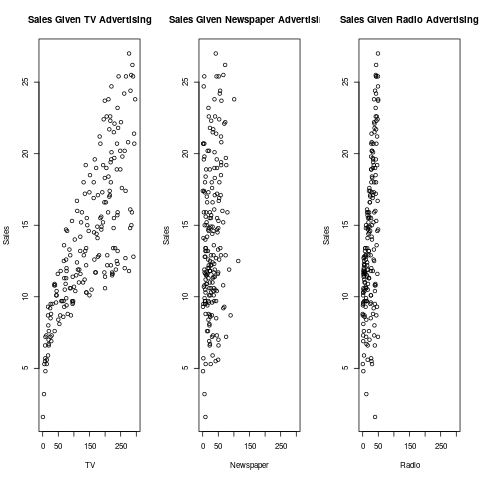
\includegraphics[width=.9\linewidth]{BaseMergedPlots02IntroData.png}
\end{center}

\begin{center}
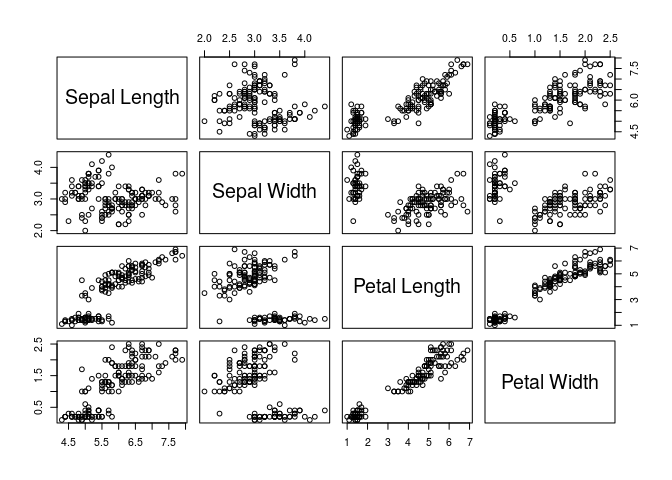
\includegraphics[width=.9\linewidth]{02_Practical_files/figure-html/unnamed-chunk-4-1.png}
\end{center}
\item GGPlot\hfill{}\textsc{ggplot2:linear:regression}
\label{sec:org7d602a0}
\begin{enumerate}
\item Television Advertising
\label{sec:orgdd060df}
\begin{minted}[]{r}
 adv$MeanAdvertising <- rowMeans(adv[,c(!(names(adv) == "Sales"))])

 AdvTVPlot <- ggplot(data = adv, aes(x = TV, y = Sales, col = MeanAdvertising)) +
   geom_point() +
   theme_bw() +
   stat_smooth(method = 'lm', formula = y ~ poly(x, 2, raw = TRUE), se = FALSE) +
  ##stat_smooth(method = 'lm', formula = y ~ log(x), se = FALSE) +
   labs(col = "Mean Advertising", x= "TV Advertising")
print(AdvTVPlot)

  if(knitr::is_html_output()){
    ggplotly(knitr::is_latex_output())
  } else {
    AdvTVPlot
  }
\end{minted}

\begin{center}
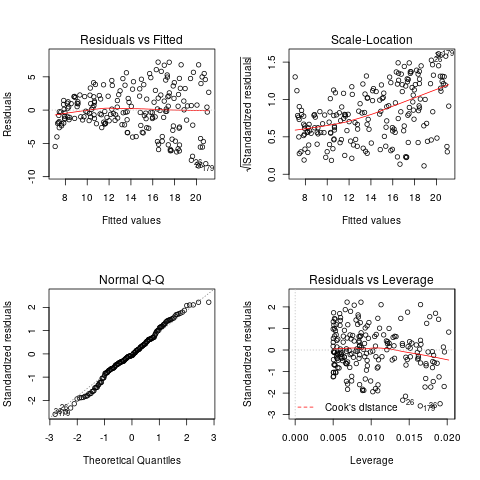
\includegraphics[width=.9\linewidth]{Intro02AdvPlotLinMod.png}
\end{center}

\item Radio Advertising
\label{sec:orgf86bbd2}
\begin{minted}[]{r}
  AdvRadPlot <- ggplot(data = adv, aes(x = Radio, y = Sales, col = MeanAdvertising)) +
    geom_point() +
    theme_bw() +
    labs(col = "Mean Advertising", x= "Radio Advertising") +
    geom_smooth(method = 'lm')

 # padv %>% ggplotly() plotly doesn't work with knitr/LaTeX so test the output and choose accordingly:
 #Thise could be combined into an interactive graph by wrapping in ggplotly(padv)

if(knitr::is_html_output()){
AdvRadPlot %>% ggplotly()
 } else {
   AdvRadPlot
 }
\end{minted}

\begin{center}
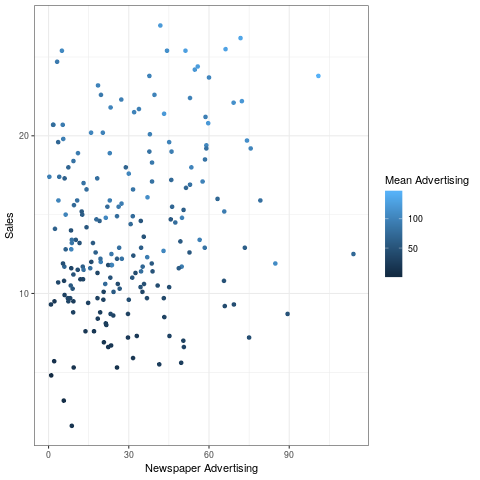
\includegraphics[width=.9\linewidth]{Intro02AdvRadioPlotLinMod.png}
\end{center}

\item Newspaper Advertising
\label{sec:org5126b6d}
\begin{minted}[]{r}
AdvNewsPlot <- ggplot(data = adv, aes(x = Newspaper, y = Sales, col = MeanAdvertising)) +
  geom_point() +
  theme_bw() +
  labs(col = "Mean Advertising", x= "Newspaper Advertising")

# padv %>% ggplotly() plotly doesn't work with knitr/LaTeX so test the output and choose accordingly:
#Thise could be combined into an interactive graph by wrapping in ggplotly(padv)

 if(knitr::is_html_output()){
AdvNewsPlot %>% ggplotly()
} else {
AdvNewsPlot
}
\end{minted}

\begin{center}
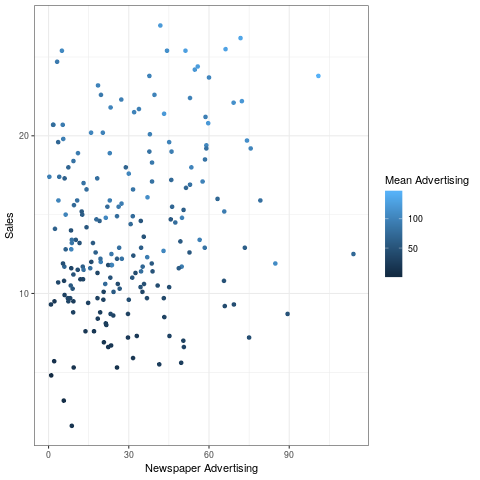
\includegraphics[width=.9\linewidth]{Intro02AdvRadioPlotLinMod.png}
\end{center}
\end{enumerate}

\item Base Plot\hfill{}\textsc{r:BasePlot}
\label{sec:orgb335fb8}
\begin{minted}[]{r}
pdom <- c(0, 300) #Plot Domain
plot(formula = Sales ~ TV, data = adv, xlim = pdom,
     main = "Sales Given TV Advertising")
\end{minted}

\begin{center}
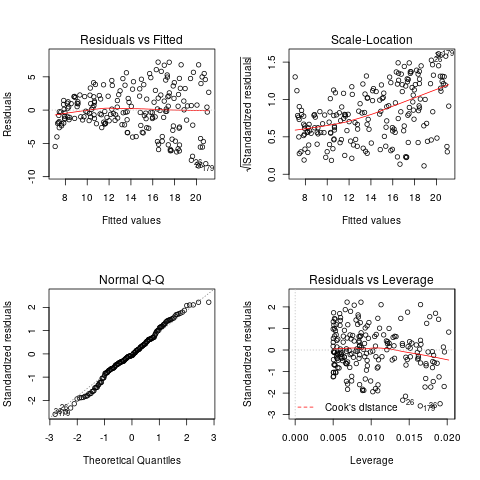
\includegraphics[width=.9\linewidth]{Intro02AdvPlotLinMod.png}
\end{center}

\begin{center}
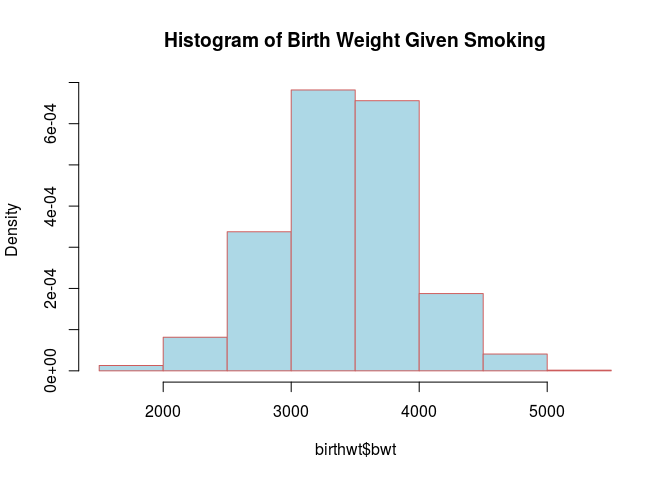
\includegraphics[width=.9\linewidth]{02_Practical_files/figure-html/unnamed-chunk-8-1.png}
\end{center}

\begin{minted}[]{r}
plot(formula = Sales ~ Newspaper, data = adv, xlim = pdom,
     main = "Sales Given Newspaper Advertising")
\end{minted}

\begin{center}
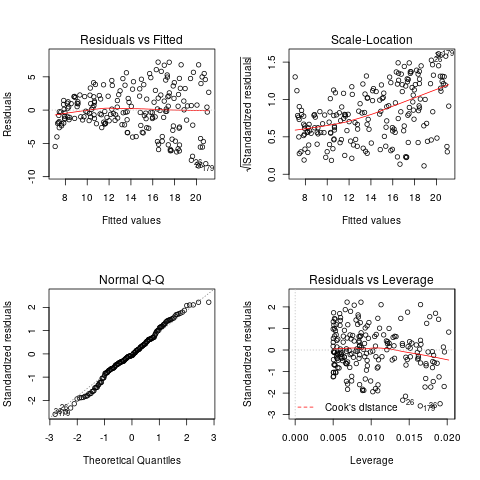
\includegraphics[width=.9\linewidth]{Intro02AdvPlotLinMod.png}
\end{center}

\begin{center}
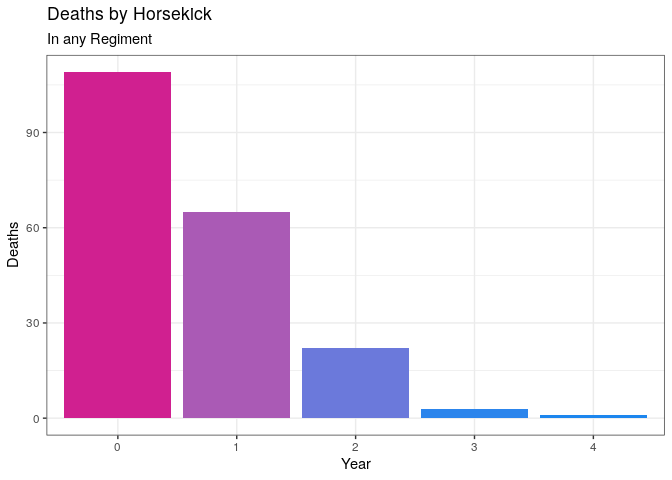
\includegraphics[width=.9\linewidth]{02_Practical_files/figure-html/unnamed-chunk-8-2.png}
\end{center}

\begin{minted}[]{r}
plot(formula = Sales ~ Radio, data = adv, xlim = pdom,
     main = "Sales Given Radio Advertising")
\end{minted}

\begin{center}
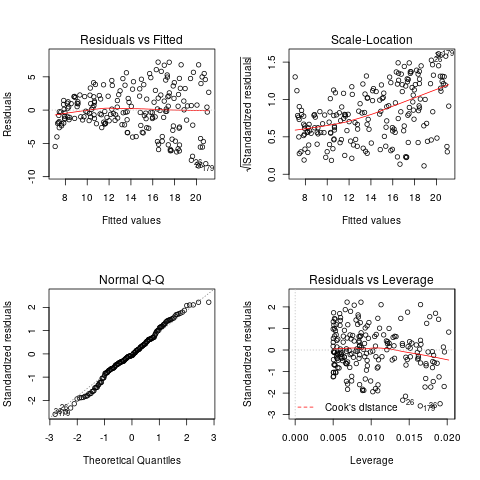
\includegraphics[width=.9\linewidth]{Intro02AdvPlotLinMod.png}
\end{center}

\begin{center}
\includegraphics[width=.9\linewidth]{02_Practical_files/figure-html/unnamed-chunk-8-3.png}
\end{center}
\end{enumerate}
\subsubsection{(c) Find the Correlation Coefficient\hfill{}\textsc{linear:regression}}
\label{sec:org1c2b8d6}
The corellation coefficient can be found by using the \texttt{cor} function, it
is a measurement of the strength of a linear relationship ranging from
-1, to 1, wherein a value of 0 would represent no relationship.

The Pearson Correlation Coeffient tends to be used over other models and
it's value is determined by:

$$
   r_{xy} = \frac{\sum^{n}_{i= 1}   \left[ x_i - \overline{x} \right] \times \left( y_i - \overline{y} \right)}{\sqrt{\sum^{n}_{i= 1}   \left[\left(  x_i - \overline{x} \right)^2 \right]} \sqrt{\sum^{n}_{i= 1}   \left[ \left( y_i- \overline{y} \right)^2 \right]}}
  $$

Some of the assumptions underlying the Correlation Coefficient
are: \footnote{\href{spss-tutorials.com/pearson-correlation-coefficient/}{Corellation
Coefficient}}

\begin{itemize}
\item Independent Observations
\item Normally distributed observations (i.e. follows a bell curve)
\item hmoscedasticity \footnote{\href{newonlinecourses.science.psu.edu/stat501}{PennState
University}}

\begin{itemize}
\item This means equal variance of observations

\begin{itemize}
\item i.e. all there is no pattern between the variables and the plot,
the points should make a rectangle, not a triangle
\end{itemize}
\end{itemize}

\item Normally distributed points
\item the points must make a straight line not a curve
\end{itemize}

the correlation coefficient in this case can be found by using
\texttt{cor(x = adv\$TV, y = adv\$Sales)} and provides that \(r \approx\) 0.78 This
might not be a meaningufl value however because the variance of the
sales appears to increase as advertising increases, if that is
overlooked however the pearson correlation coefficient provides that the
model is a reasonably strong positive linear model.
\subsubsection{(d) Assess the accuracy of the parameter estimates\hfill{}\textsc{ModelEvaluation}}
\label{sec:orga5b4169}
The parameter estimates may be returned by summarising the model with
\texttt{summary(lm)}

\begin{minted}[]{r}
lmMod <- lm(formula = Sales ~ TV, data = adv)
lmSum <- summary(lmMod)
lmSum
\end{minted}

\begin{center}
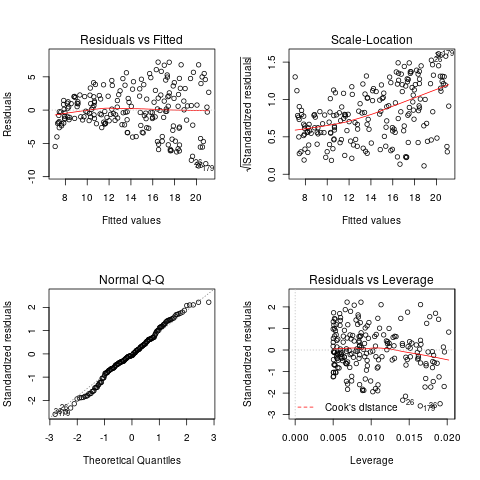
\includegraphics[width=.9\linewidth]{Intro02AdvPlotLinMod.png}
\end{center}


\begin{verbatim}
##
## Call:
## lm(formula = Sales ~ TV, data = adv)
##
## Residuals:
##     Min      1Q  Median      3Q     Max
## -8.3860 -1.9545 -0.1913  2.0671  7.2124
##
## Coefficients:
##             Estimate Std. Error t value Pr(>|t|)
## (Intercept) 7.032594   0.457843   15.36   <2e-16 ***
## TV          0.047537   0.002691   17.67   <2e-16 ***
## ---
## Signif. codes:  0 '***' 0.001 '**' 0.01 '*' 0.05 '.' 0.1 ' ' 1
##
## Residual standard error: 3.259 on 198 degrees of freedom
## Multiple R-squared:  0.6119, Adjusted R-squared:  0.6099
## F-statistic: 312.1 on 1 and 198 DF,  p-value: < 2.2e-16
\end{verbatim}

\begin{minted}[]{r}
lmSum$coefficients
\end{minted}

\begin{verbatim}
              Estimate  Std. Error  t value    Pr(>|t|)
(Intercept) 7.03259355 0.457842940 15.36028 1.40630e-35
TV          0.04753664 0.002690607 17.66763 1.46739e-42
\end{verbatim}


\begin{verbatim}
##               Estimate  Std. Error  t value    Pr(>|t|)
## (Intercept) 7.03259355 0.457842940 15.36028 1.40630e-35
## TV          0.04753664 0.002690607 17.66763 1.46739e-42
\end{verbatim}

\begin{minted}[]{r}
lmMod2 <- lm(formula = Sales ~ TV, data = adv)
\end{minted}

In this case we have:

\begin{itemize}
\item a slope of \(\beta_1 \approx\) 0.048 \(\pm\) 0.0027
\item an Intercept of \(\beta_0 \approx\) 7 \(\pm\) 0.46
\end{itemize}

The standard deviation of a statistic used as an estimator of a
population parameter is often referred to as the \textbf{standard error of the
estimator (S.E.)}; it is the \(\pm\) values specified above:

\begin{itemize}
\item Standard Error of Slope Coefficient
\(\sigma_{\beta_1} = s\sqrt{\frac{1}{n}+ \frac{\overline{x}^2}{SS_x}} = 0.00027\)
\item Standard Errof of Intercept Coefficint
\(\sigma_{\beta_0} = \frac{s}{\sqrt{SS_x}} = 0.46\)
\end{itemize}

Where:

\begin{itemize}
\item \(s\) is the sample standard deviation (OF WHAT?)
\item \(SS_x = \sum^{n}_{i= 1} \left[ x^2_i \right] - n\cdot \left( \overline{x} \right)^2\)
\item s is the sample standard deviation of \(x\)
\item because the sample standard deiation of \(x\) predicts the deviation of
\(y\) anyway
\end{itemize}

You may also have the standard deviation of the residuals (the distance
along the y-axis of a point from the regression line), this is known as
the \textbf{Residual Standard Error} and is calculated via the \emph{Ordinary Least
Squares Method} \footnote{i.e. chosing \(\beta_0\) and \(\beta_1\) to minimise
\(\left(\textbf{RSS} = \sum^{n}_{i= 1} \left[ \left( y_i - \hat{y_i} \right)^2 \right] \right)\)}, it is is given by:

\begin{align}
 \sigma_{\varepsilon} = S.E. & = \sqrt{\frac{\textbf{RSS}}{N}}\\
 \ \\
 &= \sqrt{\frac{\sum^{n}_{i= 1}   \left[ \left( y_i - \hat{y}_i \right)^2 \right]}{N}}
\end{align}

Which you'll notice is identical to the \textbf{\emph{RMSE}}.

so by the emperical method \(2\times \text{S.E.}\) would represent a 95\%
confidence interval (rather than prediction interval) of the expected
\$y\$-values. Drawing such a confidence interval:

\begin{minted}[]{r}
paramint <- confint(object = lm(adv$Sales ~ adv$TV), level = 0.95) %>% signif(2)
paramint
\end{minted}

\begin{verbatim}
##             2.5 % 97.5 %
## (Intercept) 6.100  7.900
## adv$TV      0.042  0.053
\end{verbatim}

So drawing from this we could expect, with only a 5\% probability of
incorrectly rejecting the null hypothesis that there is no relationship,
that in the absence of advertising, the TV sales to fall between 6.1 and
7.9.

With the same degree and type of certainty it could also be oncluded
that for every \$1000 increase in advertising, the tv sales will increase
by between 42 and 53.
\begin{enumerate}
\item (f) Test the significance of the slope of the linear model
\label{sec:orgc6ada8f}
If it is appropriate to fit a linear model to data, then we can test for
correlation between the data points by considering whether or not the
slope value is non-zero \(\beta_1 \neq 0\), this is because a zero
coefficient would be such that the model would predict
\(Y = C + \varepsilon\), this means that \(X\) is not a feature/predictor of
\(Y\), however \(Y\) may still be a function of (or rather response variable
of) other values other factors that are 'behind the scenes'.\footnote{Refer to page 67 of the text book, section [3.1.2]}

So our hypotheses would be:

\begin{align}
H_0 : \enspace \beta_1 &= 0 \qquad ( \small {\text{ The null hypothesis is that nothings related}})\\
H_1 : \enspace \beta_1 &= 1
\end{align}

So our interest is to determine how far from 0 our expected \(\beta_1\)
value needs to be from 0 for us to conclude

\begin{quote}
The expected value of \(\beta_1\) is so far from zero we can conclude
that it it's not zero at some significance level \(^{\dagger}\)"
\end{quote}

\begin{quote}


\#+BEGIN\textsubscript{QUOTE}
  \emph{\(\dagger\) at some low probability of incorrectly rejecting the null
  hypothesis}
\end{quote}
\#+END\textsubscript{QUOTE}

The problem is defining how far from zero is far enough, for this we use
the expected distance from the regression line, the standard error from
above, a value observed observed too many standard deviations to the
right of the mean are not very likely too occur.
\begin{enumerate}
\item Choosing a Parametric method
\label{sec:orgc595d81}
A statistical method that relies on an underlying assumption of the
statistical distribution of the data is known as a a parametric method,
in this case, it is a fundamental assumption of \textbf{Ordinary Least Squares}
Linear regression that the data is normally distributed.\footnote{Mendenhall, \emph{Introduction to Probability \& Statistics} p. 254
[7.4]}

This is a situation where we use the \emph{Student's t-test} because this is
a sample, and the population standard deviation \(\left( \sigma \right)\)
is not known and hence the confidence interval for the mean must be made
broader in order to account for the fact that the sample standard
deviation \(s\) is being used to estimate \(\sigma\)

because the sampled population is normally distributed, the sampling
distribution of \(\bar{x}\) will be normally distributed \footnote{By the Central Limit Theorem}
(regardless of sample size) and centred about \(\mu\) with a a standard
deviation of \(\frac{\sigma}{\sqrt{n}}\). If the population was non-normal
the sampling distribution will be approximately normal for \(n\geq 30\).

Because \(\frac{\sigma}{n}\) is the standard deviation of the the sample
mean \(\bar{x}\) it is reffered to as the \textbf{Standard Error of the
mean} \footnote{Mendenhall, \emph{Introduction to Probability \& Statistics} p. 254
[7.4]}, so we could calculate the critical value along the
standard normal distribution corresponding to the the sampling
distribution in order to determine probabilities, however, \(\sigma\) is
unknown and using \(s\) instead will not create a normal distribution, the
distriution it creates is Gosset's \textbf{Student's t-distribution} \footnote{Mendenhall, \emph{Introduction to Probability \& Statistics} p. 254
[7.4]}:

\begin{align}
  t = \frac{\overline{x}- \mu}{\frac{s}{\sqrt{n}}}
\end{align}

So in this case our test statistic will be:

\begin{align}
t = \frac{\hat{\beta}_1- 0}{\text{SE}\left( \hat{\beta}_1 \right)}
\end{align}

In order to perform this test in R we can use \texttt{qnorm} and \texttt{qt} to return
critical values, \texttt{t.test} will perform a hypothesis test directly from
input data but that's not suitable here.

\begin{minted}[]{r}
tcritval <- qt(p = 0.05,df =nrow(adv)-2 )
tcritval %>% signif(2)
\end{minted}

\begin{verbatim}
## [1] -1.7
\end{verbatim}

So the critical t-value is -1.7 and from the summary call from before we
have that the t-statistic is 17, which far exceeds this, as a matter of
fact further over to the right the p-value is reported at
\(\alpha = 10^{-16}\).

In practice you'd just read off the \emph{p}-values and pick the ones with
\texttt{*} to the right of them, the more \texttt{*} the more significance.

Hence we reject the hypothesis that no relationship exists at an
extremely low probability of incorrectly doing so (i.e. low probability
of commiting type 1 error).
\end{enumerate}
\item (g) Plot the straight line within the scatter plot and comment
\label{sec:org9374a53}
\begin{enumerate}
\item Base Plot
\label{sec:orgccf5811}
In order to plot this inside base packages, feed the model object,
i.e. =lm(Y\textasciitilde{}X)= inside a call to \texttt{abline()} in order to plot the model
over the top of the base plot, so all together it might look
like: \footnote{\href{https://stats.stackexchange.com/a/11028}{\texttt{na.exclude} will pad
values extracted so lengths are the same, \texttt{na.omit} will not}}

\begin{verbatim}
Form <- Sales ~ TV
Lmodel <- lm(formula = Form, data = adv, na.action = na.exclude)
plot(Form, data = adv)
abline(Lmodel)
\end{verbatim}

Or you could do it like this even, but I think the way above is better
syntax because it will behave better with 'predict' function and follows
\texttt{tidyverse} syntax

\begin{verbatim}
Lmodel <- lm(adv$Sales ~ adv$TV)
plot(x = adv$TV, y = adv$Sales)
abline(a = Lmodel$coefficients[1], b = Lmodel$coefficients[2])
\end{verbatim}

\begin{minted}[]{r}
plot(formula = Sales ~ TV, data = adv, xlim = pdom,
     main = "Sales Given TV Advertising")

abline(lmMod)
\end{minted}

\begin{center}
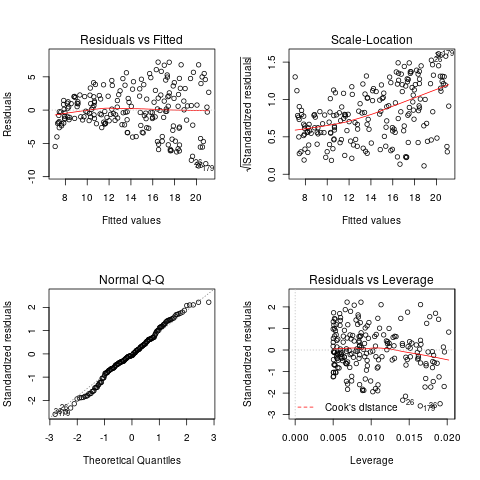
\includegraphics[width=.9\linewidth]{Intro02AdvPlotLinMod.png}
\end{center}

\begin{center}
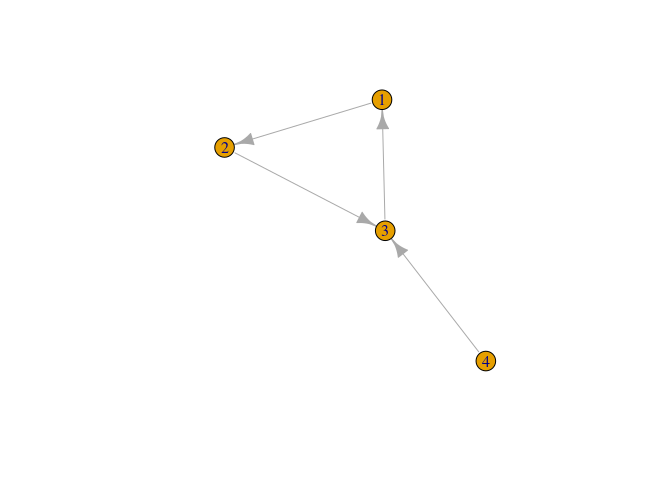
\includegraphics[width=.9\linewidth]{02_Practical_files/figure-html/unnamed-chunk-12-1.png}
\end{center}
\item GGplot\hfill{}\textsc{linear:regression:ggplot2}
\label{sec:orgce72af0}
\begin{minted}[]{r}
AdvTVPlot <- ggplot(data = adv, aes(x = TV, y = Sales, col = MeanAdvertising)) +
  geom_point() +
  theme_bw() +
  stat_smooth(method = 'lm', formula = y ~ x, se = FALSE)

AdvTVPlot
\end{minted}

\begin{center}
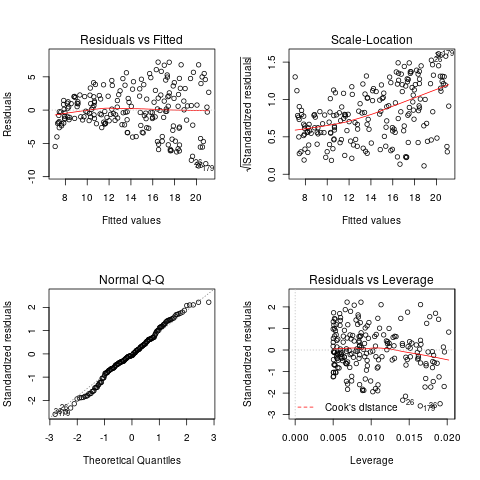
\includegraphics[width=.9\linewidth]{Intro02AdvPlotLinMod.png}
\end{center}

\begin{center}
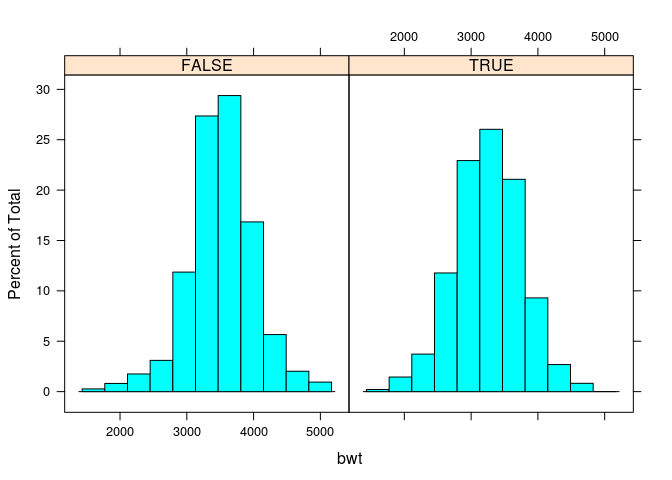
\includegraphics[width=.9\linewidth]{02_Practical_files/figure-html/unnamed-chunk-13-1.png}
\end{center}

If we needed to feed ggplot a specific model we could do that like this,
but it's a whole thing to do and you'd probably rather not do it this
way, but if you really really need to

\begin{minted}[]{r}
AdvTVPlot <- ggplot(data = adv, aes(x = TV, y = Sales, col = MeanAdvertising)) +
  geom_point() +
  theme_bw() +
  stat_smooth(
      method = "lm",
      mapping = aes( y = predict(lmMod)
                     )
      )

AdvTVPlot
\end{minted}

\begin{center}
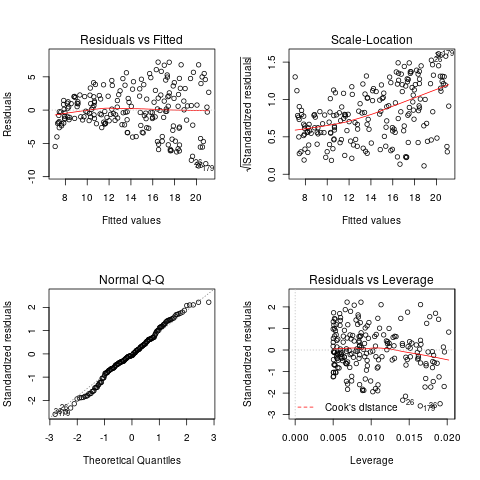
\includegraphics[width=.9\linewidth]{Intro02AdvPlotLinMod.png}
\end{center}

\begin{center}
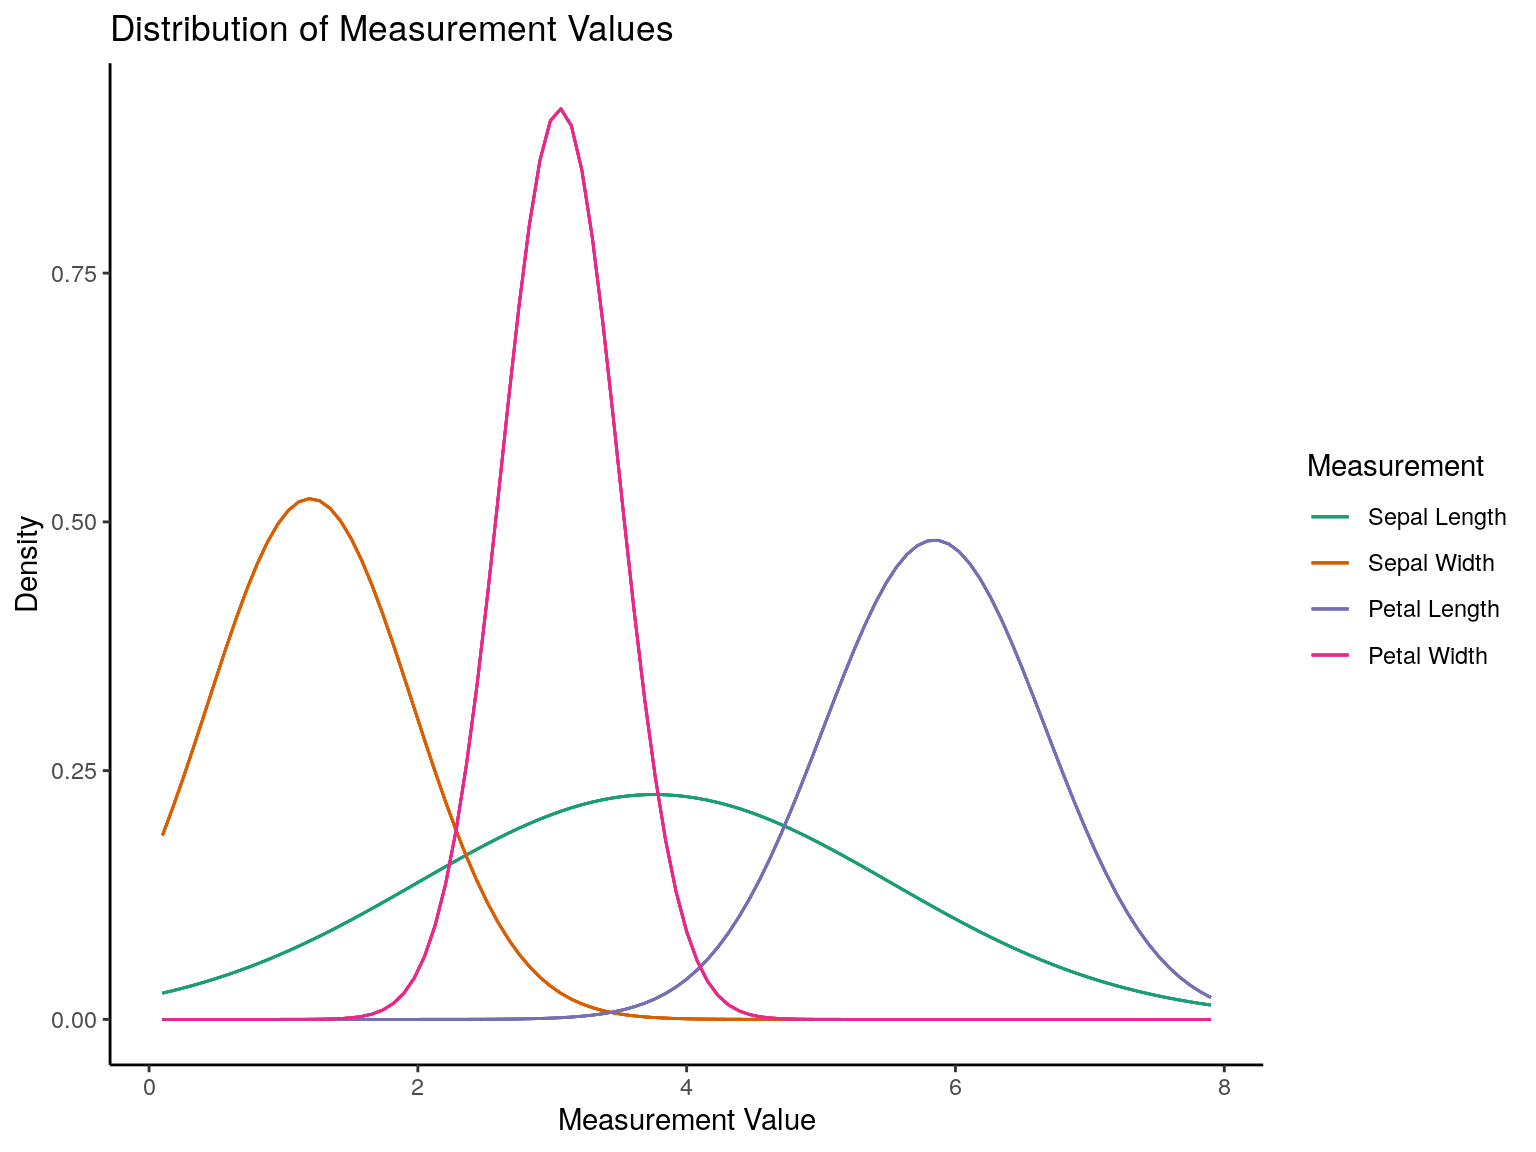
\includegraphics[width=.9\linewidth]{02_Practical_files/figure-html/unnamed-chunk-14-1.png}
\end{center}
\end{enumerate}
\item (h) Assess the overall accuracy of the model
\label{sec:org9c8dfc0}
The model can be assed by considering the:

\begin{itemize}
\item Coefficient of determination \(R^2\) which is the proportion of variance
in the data that is explained by the model
\item Only in the case of simple linear regression is \(R^2 = (r)^2\)
\item The Residual Standard Error is the standard deviation of the
residuals, i.e. it is the expected distance between each point to the
regression line, taken along the \$y\$-axis.
\end{itemize}
\begin{enumerate}
\item Terminology
\label{sec:org971a574}
The texbook makes, in my opinion, a mistake in that it refers to the the
\emph{Root Mean Square Error} (\textbf{\emph{RMSE}}) as the \emph{Residual Standard Error}
(\textbf{\emph{RSE}}) \footnote{Refer to Page 69 of the TB for RMSE definition, the TB divides
by DF which is probably more correct that dividing by sample
size.}, this is true, the standard error of the residuals
(\(\varepsilon\)) would be the RMSE, so we would have \textbf{\emph{RMSE}}
\(= \sigma_{\varepsilon}\), that's fine.

The issue is there is another common term used called the \emph{Relative
Squared Error} (\textbf{\emph{RSE}}) is often used \footnote{\href{https://www.saedsayad.com/model\_evaluation\_r.htm}{An
Introduction to Data Science : Model Evaluation - Regression}} and so this is hence
ambiguous, hence forth I will:

\begin{itemize}
\item Refer to the Standard Error of the residuals (\(\sigma_{varepsilon}\))
as \textbf{\emph{RMSE}}:

\begin{itemize}
\item \(\text{RMSE} = \sqrt{\frac{\sum{\varepsilon ^2}}{n}}\)
\end{itemize}

\item Refer to the Relative Standard Error as \textbf{\emph{RSE}}

\begin{itemize}
\item \(\text{RSE} = \frac{\sigma_{\varepsilon} ^2}{\sigma_y ^2} = \frac{\sum{\left( y-\hat{y} \right)^2 }}{ \sum{ \left( y-\bar{y} \right)^2 } }\)

\begin{itemize}
\item The advantage to the RSE is that it can be compared between models
with different units, whereas the RMSE cannot, just another tool
in the belt I suppose.
\end{itemize}
\end{itemize}
\end{itemize}
\item Root Mean Square Error\hfill{}\textsc{LossFunction}
\label{sec:orge202012}
Recall that the model was of the form
\(Y = \beta_1 X + \beta_0 + \varepsilon\), the \textbf{\emph{RMSE}} (\emph{Root Mean Square
Error}) is the standard deviation of \(\varepsilon\) as measured along the
\$Y\$-axis:

\begin{align}
 \sigma_{\varepsilon} =  \sqrt{\frac{\sum^{n}_{i= 1}   \left[ \left( y_i - \hat{y}_i \right)^2 \right]}{N}}
\end{align}

This value can be returned from R by investigating the anova table:

\begin{minted}[]{r}
anova(lmMod)
\end{minted}

\begin{verbatim}
## Analysis of Variance Table
##
## Response: Sales
##            Df Sum Sq Mean Sq F value    Pr(>F)
## TV          1 3314.6  3314.6  312.14 < 2.2e-16 ***
## Residuals 198 2102.5    10.6
## ---
## Signif. codes:  0 '***' 0.001 '**' 0.01 '*' 0.05 '.' 0.1 ' ' 1
\end{verbatim}

From the \emph{ANOVA} table it can be seen that the average squared residual
is 10.6

\begin{align}
\text{mean}\left( \varepsilon^2\right) &= 10.6\\
\implies \frac{1}{n} \cdot \sum^{n}_{i=1} \left[ \varepsilon_i \right] & =10.6\\
\implies \frac{1}{n} \cdot \sum^{n}_{i=1} \left[ \left( \hat{y}_i - y_i \right)^2 \right] & =10.6\\
\implies \sqrt{\frac{1}{n} \cdot \sum^{n}_{i=1} \left[ \left( \hat{y}_i - y_i \right)^2 \right] } & = 3.2\\
\ \\
\implies \sigma_{\varepsilon} &= 3.2
\end{align}

Thus we may conclude that we expect the model to predict the sales
within \(\pm\) 3.2 units, which is quite predictive and hence useful.
\item Coefficient of Determination
\label{sec:orgd6856d0}
The coefficient of determination is the proportion of variation within
the model that is explained by the model:

\begin{align}
R^2 &= \frac{TSS-RSS}{TSS}\\
&= \frac{3315}{3315+2103}\\
\ \\
&= 0.612
\end{align}

In practice we would simply extract the coefficient of determination
(\(R^2\)) from the model-summary:

\begin{minted}[]{r}
lmSum$r.squared %>% round(3) %>% percent()
\end{minted}

\begin{verbatim}
## [1] "61.2%"
\end{verbatim}

This value suggests that a reasonable amount of the variation is
explained by the model, but perhaps a non-linear model could explain
more of the variance. (be careful a significant coefficient of
determination doesn't necessarily mean that the slope is significantly
different from 0)
\item Residual Analysis
\label{sec:org14d95a7}
\begin{minted}[]{r}
layout(matrix(1:4, nrow = 2))
plot(lmMod)
\end{minted}

\begin{center}
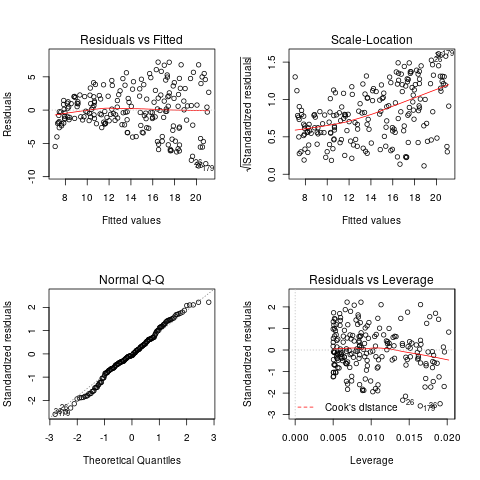
\includegraphics[width=.9\linewidth]{Intro02AdvPlotLinMod.png}
\end{center}

\begin{center}
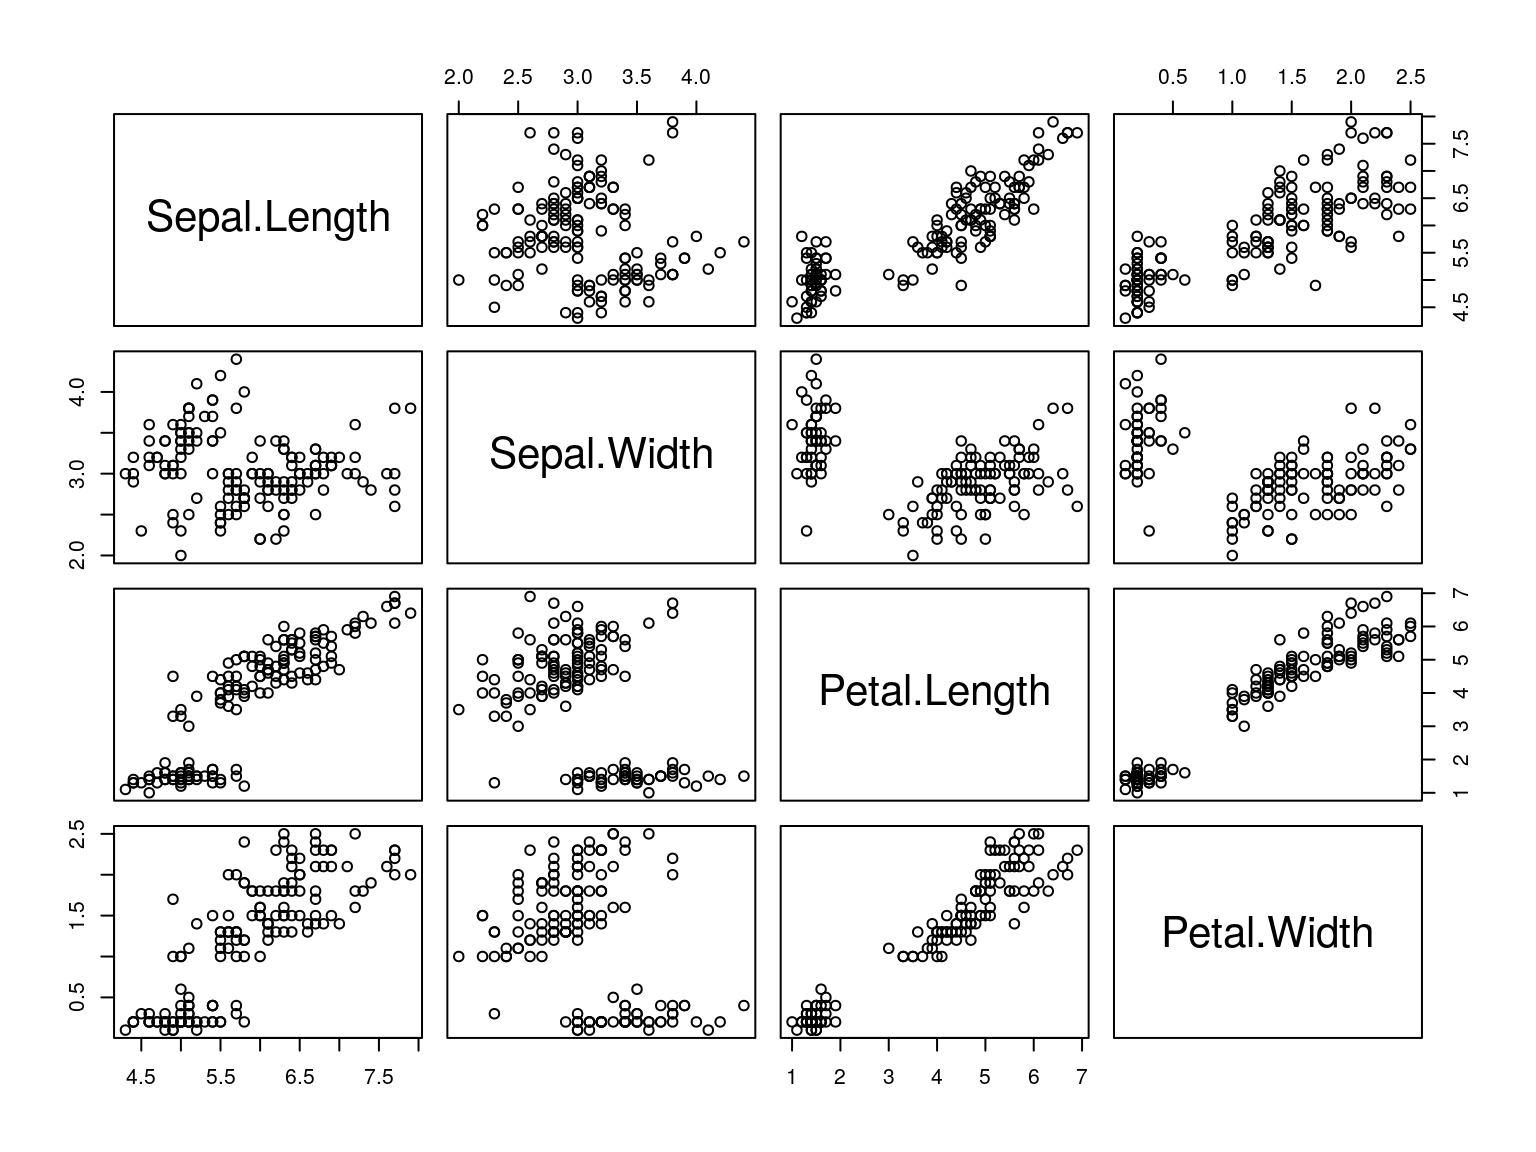
\includegraphics[width=.9\linewidth]{02_Practical_files/figure-html/unnamed-chunk-17-1.png}
\end{center}

\begin{itemize}
\item The residual plot does not appear to normally distributed, there is a
slight logarithmic trend, this violates assumptions of the linear
model undermining the predictive capacity of the model in this case.
\item The variance is also non-constant, for a linear model to be used in
must be homoscedastic (i.e. constant variance), this is not the case
implying that the assumptions of the linear model have been violated
and hence this model may not be appropriate \footnote{refer to page 96 of the TB, log or exp transforming may be
appropriate here, the data is not homosdcedastic and is hence
said to be heteroscedastic. \#\#\#\# How to use predict}
\item the standardised residuals should be normally distriuted with a mean
of 0 and standard deviation of 1, whilst the standard deviation
appears acceptable, the standardised residuals are centred around
\(\approx 3/4\) with a positive upward slope violating the assumption of
normality.
\item The normal Q-Q plot is a straight line so actually the data is
probably normally distributed, the only issue is the
heteroscedasticity of the data.
\item The Cook's Distance plot suggests that there are some points with a
high amount of leverage, so perhaps there are some outliers or perhaps
the increasing variance is undermining the appropriateness of the
model.
\end{itemize}
\end{enumerate}
\item (i) Use the model to make predictions
\label{sec:org8cb53e8}
When making predictions is important to ensure that the names of a data
frame are \texttt{syntactically correct}, otherwise you will have a bad day
trying to get predict to work and ggplot2 to work because specifying the
data frame names in a formula will be difficult, make sure that names
are always syntactically valid.

what is important is you create your model with the correct syntax, if
you create your model like this:

\begin{verbatim}
mymodelWRONG <- lm(adv$Sales ~ adv$TV)
\end{verbatim}

you won't be able to predict data like this:

\begin{verbatim}
predict(object = lmMod, newdata = data.frame("TV" = 300))
\end{verbatim}

you'll just get an error that says
\texttt{'newdata' had 1 row but variables found have 200 rows}, you have to
give the variables corresponding names so that the model object can save
them for later and make the connection, for instance, if inspect the
terms from above you will get:

\begin{verbatim}
mymodelWRONG[["terms"]]
\end{verbatim}

which outputs, at the tail end:

\begin{verbatim}
adv$Sales    adv$TV
"numeric" "numeric"
\end{verbatim}

where as if you create the model like this:

\begin{verbatim}
lmModCORRECT <- lm(formula = Sales ~ TV, data = adv)
predict(object = lmModCORRECT, newdata = data.frame("TV" = 300))
\end{verbatim}

and inspect the terms with:

\begin{verbatim}
lmModCORRECT[["terms"]]
\end{verbatim}

you will get this as output

\begin{verbatim}
  Sales        TV
"numeric" "numeric"
\end{verbatim}

where \texttt{Sales} and \texttt{TV} are the outputs of \texttt{names(adv)} and so I can use
that when I use predict. You should not use \texttt{attach} it will cause
problems later, however, it can be nice to use attach just before a
predict call to get auto completed names and then remove attach and
re-execute the script .

So always use the \texttt{lm(formula = Y\textasciitilde{}X, data = myDF)} because it works the
best; you have to use the same syntax/format when using predict or
ggplot anyway so there's no reason not to use the same syntax throughout
anyway.

Also the lecturer said to use lists, I reckon use data frames because
that way your \texttt{newdata} matches the input data one-to-one, moreover:

\begin{itemize}
\item It makes it far simpler to assign names, because again, the
input/ouptu data will all be the same format
\item when creating \emph{Lasso} Regression Models you have to use matrices as
input data and it's easier to set your workflow up to go from
dataframe to matrix (You have to do this in predictive modelling)
\end{itemize}
\begin{enumerate}
\item Predict the Data
\label{sec:org83ed81c}
\begin{enumerate}
\item One Point
\label{sec:orgb6099fd}
\begin{minted}[]{r}
input = 3
output <- predict(object = lmMod, newdata = data.frame("TV" = 3))
predDatasingle <- data.frame(input, output)
names(predDatasingle) <- names(adv[c(1,4)])

print(predDatasingle)
\end{minted}

\begin{verbatim}
##   TV    Sales
## 1  3 7.175203
\end{verbatim}
\item Multiple points
\label{sec:org40327bb}
\begin{minted}[]{r}
input <- seq(from = 100, to = 900, by = 100)
output <- predict(object = lmMod, newdata = data.frame("TV" = input))

predDF <- data.frame(input, output)
names(predDF) <- names(adv[c(1,4)])
predDF
\end{minted}

\begin{verbatim}
##    TV    Sales
## 1 100 11.78626
## 2 200 16.53992
## 3 300 21.29359
## 4 400 26.04725
## 5 500 30.80091
## 6 600 35.55458
## 7 700 40.30824
## 8 800 45.06191
## 9 900 49.81557
\end{verbatim}
\end{enumerate}
\end{enumerate}
\end{enumerate}
\subsection{Question 02}
\label{sec:orgdb41fa8}
\subsubsection{(a) Upload the Auto Dataset and explore it.}
\label{sec:org31ab181}
\subsubsection{(b) Construct scatter plots to visualize the relationship between}
\label{sec:org9a78e63}
mpg and displacement, weight and accellertion:
:CUSTOM\textsubscript{ID}: b-construct-scatter-plots-to-visualize-the-relationship-between-mpg-and-displacement-weight-and-accellertion
\subsubsection{Repeat the analysis in Q1 (c) to (i) using mpg and weight.}
\label{sec:orgc666646}
\section{Multiple Linear Regression}
\label{sec:org6309502}
Material of Tue 19 March2019, week 3

\subsection{Question 01 - Multiple Linear Regression}
\label{sec:orgc6c919e}
\subsubsection{Load Packages}
\label{sec:orgbb30466}

\begin{minted}[]{r}
# Load Packages
if(require('pacman')){
  library('pacman')
}else{
  install.packages('pacman')
  library('pacman')
}

pacman::p_load(caret, scales, ggplot2, rmarkdown, shiny, ISLR, class, BiocManager,
               corrplot, plotly, tidyverse, latex2exp, stringr, reshape2, cowplot, ggpubr,
               rstudioapi, wesanderson, RColorBrewer, colorspace, gridExtra, grid, car,
               boot, colourpicker, tree, ggtree, mise, rpart, rpart.plot, knitr, MASS,
               magrittr, EnvStats,tidyverse,tidyr,devtools, bookdown, leaps, car, clipr,
               tikzDevice, e1071)



mise()
set.seed(0932)
\end{minted}

\subsubsection{(a) Upload the data "Advertising.csv" and explore it.\hfill{}\textsc{ATTACH}}
\label{sec:org80f4599}
First import the data and investigate it:


\begin{minted}[]{r}
adv <- read.csv(file = "../.././data/83/4c42c3-8dd8-4fef-b402-7e341764d5e9/Advertising.csv", header = TRUE, sep = ",")
\end{minted}

\begin{minted}[]{r}
head(adv)
\end{minted}

\begin{verbatim}
##      TV Radio Newspaper Sales
## 1 230.1  37.8      69.2  22.1
## 2  44.5  39.3      45.1  10.4
## 3  17.2  45.9      69.3   9.3
## 4 151.5  41.3      58.5  18.5
## 5 180.8  10.8      58.4  12.9
## 6   8.7  48.9      75.0   7.2
\end{verbatim}

\begin{minted}[]{r}
writeLines("\n")
\end{minted}

\begin{minted}[]{r}
print("***Dimensions***")
\end{minted}

\begin{verbatim}
## [1] "***Dimensions***"
\end{verbatim}

\begin{minted}[]{r}
writeLines("\n")
\end{minted}

\begin{minted}[]{r}
dim(adv)
\end{minted}

\begin{verbatim}
## [1] 200   4
\end{verbatim}

\begin{minted}[]{r}
writeLines("\n")
\end{minted}

\begin{minted}[]{r}
print("***Summary***")
\end{minted}

\begin{verbatim}
## [1] "***Summary***"
\end{verbatim}

\begin{minted}[]{r}
writeLines("\n")
\end{minted}

\begin{minted}[]{r}
summary(adv)
\end{minted}

\begin{verbatim}
##        TV             Radio          Newspaper          Sales      
##  Min.   :  0.70   Min.   : 0.000   Min.   :  0.30   Min.   : 1.60  
##  1st Qu.: 74.38   1st Qu.: 9.975   1st Qu.: 12.75   1st Qu.:10.38  
##  Median :149.75   Median :22.900   Median : 25.75   Median :12.90  
##  Mean   :147.04   Mean   :23.264   Mean   : 30.55   Mean   :14.02  
##  3rd Qu.:218.82   3rd Qu.:36.525   3rd Qu.: 45.10   3rd Qu.:17.40  
##  Max.   :296.40   Max.   :49.600   Max.   :114.00   Max.   :27.00
\end{verbatim}

\begin{minted}[]{r}
writeLines("\n")
\end{minted}

\begin{minted}[]{r}
print("***Structure***")
\end{minted}

\begin{verbatim}
## [1] "***Structure***"
\end{verbatim}

\begin{minted}[]{r}
writeLines("\n")
\end{minted}

\begin{minted}[]{r}
str(adv)
\end{minted}

\begin{verbatim}
## 'data.frame':    200 obs. of  4 variables:
##  $ TV       : num  230.1 44.5 17.2 151.5 180.8 ...
##  $ Radio    : num  37.8 39.3 45.9 41.3 10.8 48.9 32.8 19.6 2.1 2.6 ...
##  $ Newspaper: num  69.2 45.1 69.3 58.5 58.4 75 23.5 11.6 1 21.2 ...
##  $ Sales    : num  22.1 10.4 9.3 18.5 12.9 7.2 11.8 13.2 4.8 10.6 ...
\end{verbatim}

\begin{minted}[]{r}
writeLines("\n")
\end{minted}

Fom this we can tell that there is one output, with 3 input values and
200 Observations.

\subsubsection{}
\label{sec:org242e409}

\subsubsection{(b) Find the Covariance and Correlation Matrix of Sales, TV, Radio}
\label{sec:orgf99150e}
and Newspaper.
:CUSTOM\textsubscript{ID}: b-find-the-covariance-and-correlation-matrix-of-sales-tv-radio-and-newspaper.
:CLASS: tabset

\begin{enumerate}
\item Base Packages
\label{sec:orgd8baea4}
\begin{minted}[]{r}
pairs(x = adv)
\end{minted}

\begin{center}
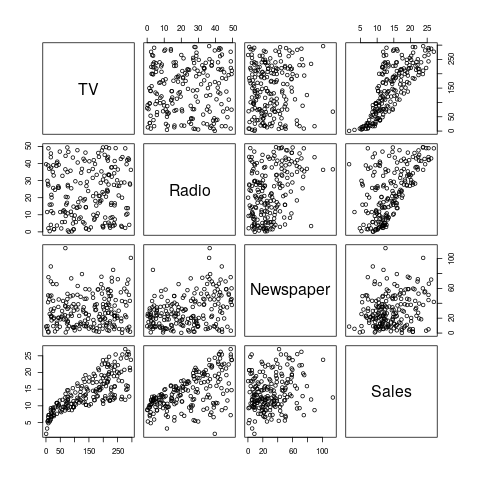
\includegraphics[width=.9\linewidth]{AdvCorPlotMultLinReg.png}
\end{center}

\begin{center}
\includegraphics[width=.9\linewidth]{./attachments/MultLinReg727unnamed-chunk-4-1.png}
\end{center}

\item corrplot
\label{sec:org4e7e442}
In order to use \texttt{corrplot} first create a correlation matrix using
\texttt{cor(adv)} then feed that matrix to \texttt{corrplot} with the command
\texttt{corrplot(cor(adv))}

\begin{minted}[]{r}
# coriris <- cor(iris[,!(names(iris) == "Species")])
# corrplot(method = 'ellipse', type = 'lower', corr = coriris)

corMat <- cor(x = adv)
corrplot(corr = corMat, method = "ellipse", type = "lower")
\end{minted}

\begin{center}
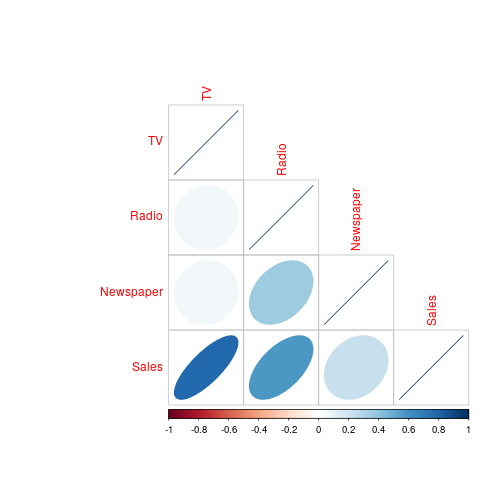
\includegraphics[width=.9\linewidth]{CorrPlotMultLinReg.png}
\end{center}

\begin{center}
\includegraphics[width=.9\linewidth]{./attachments/MultLinReg727unnamed-chunk-5-1.png}
\end{center}

\begin{HTML}
</div>
\end{HTML}

From this we can see that there is a significant amount of correlation
between Radio and newspaper (moreso even that newspaper and sales), we
should consider this variable interaction when decide upon our model
\end{enumerate}

\subsubsection{(c) Construct the multiple linear regression model and find the}
\label{sec:org2d0fda3}
least square estimates of the model
:CUSTOM\textsubscript{ID}: c-construct-the-multiple-linear-regression-model-and-find-the-least-square-estimates-of-the-model

A multiple linear regression would give the model:

\begin{minted}[]{r}
advModMult <- lm(formula = Sales ~ TV + Radio + Newspaper, data = adv)
advModMult
\end{minted}

\begin{verbatim}
## 
## Call:
## lm(formula = Sales ~ TV + Radio + Newspaper, data = adv)
## 
## Coefficients:
## (Intercept)           TV        Radio    Newspaper  
##    2.938889     0.045765     0.188530    -0.001037
\end{verbatim}

This gives that the appropriate linear model is:

$$
  Y_{Sales} = 0.0458 \times \text{TV} + 0.19 \times \text{Radio} - 0.001 \times \text{Newspaper}
  $$ the fact that Newspaper has a negative coefficient despite being
positively correlated with sales is indicative of the weak effect
newspaper advertising has on sales as well as the interaction between
newspaper and sales.

from this it can be \#\#\# (d) Test the significance of the parameters and
find the resulting model to model Sales in terms of advertising modes,
TV, Radio and Newspaper. First Summarise the Model:

\begin{minted}[]{r}
advModMult %>% summary()
\end{minted}

\begin{verbatim}
## 
## Call:
## lm(formula = Sales ~ TV + Radio + Newspaper, data = adv)
## 
## Residuals:
##     Min      1Q  Median      3Q     Max 
## -8.8277 -0.8908  0.2418  1.1893  2.8292 
## 
## Coefficients:
##              Estimate Std. Error t value Pr(>|t|)    
## (Intercept)  2.938889   0.311908   9.422   <2e-16 ***
## TV           0.045765   0.001395  32.809   <2e-16 ***
## Radio        0.188530   0.008611  21.893   <2e-16 ***
## Newspaper   -0.001037   0.005871  -0.177     0.86    
## ---
## Signif. codes:  0 '***' 0.001 '**' 0.01 '*' 0.05 '.' 0.1 ' ' 1
## 
## Residual standard error: 1.686 on 196 degrees of freedom
## Multiple R-squared:  0.8972, Adjusted R-squared:  0.8956 
## F-statistic: 570.3 on 3 and 196 DF,  p-value: < 2.2e-16
\end{verbatim}

A summary of the model provides that given the hypothesis test: $$
  H_0: \enspace \beta_i = 0\\
  H_a: \enspace \beta_i \neq 0 \\
  \qquad \qquad \qquad \qquad \forall i \in \mathbb{N}
  $$

There would be an extremely low probability of incorrectly rejecting the
null hypothesis that the given a linear model the coefficients would be
zero, hence it is accepted that the coefficients are non-zero except for
newspaper advertising.

There is a high probability of incorrectly rejecting the null-hypothesis
and hence that should not be rejected and the nespaper advertising
should not be seen as significant predictor for sales in this linear
model.

It is hence approprate to remove, via backwards selection, Newspaper
from the model, which gives:

\begin{minted}[]{r}
## Calculate Power??

# n <-  length(adv)
# sigma <-  sd(adv$Newspaper)
# sem = sigma/sqrt(n)
# alpha <-  0.05
# mu0 <- 0
# q <- qnorm(p = 0.005, mean = mu0, sd = sem);q
# mu <- q # assumed actual mean value
# pnorm(q, mean = mu, sd = sem, lower.tail = FALSE)
\end{minted}

\begin{minted}[]{r}
advModMultb1 <- lm(formula = Sales ~ TV + Radio, data = adv)
advModMultb1
\end{minted}

\begin{verbatim}
## 
## Call:
## lm(formula = Sales ~ TV + Radio, data = adv)
## 
## Coefficients:
## (Intercept)           TV        Radio  
##     2.92110      0.04575      0.18799
\end{verbatim}

\begin{minted}[]{r}
advModMultb1.sum <- summary(advModMultb1)
\end{minted}

$$
  \text{Sales} = 0.045 \times \text{TV} + 0.19 \times \text{Radio} + 2.9211
  $$

All parameters are highly significant and hence the model is deemed
adequate, the model explains 100\% of the variation, this can be found by
appending \texttt{\$r.squared} to the model object.

\subsubsection{(e) Assess the overall accuracy of the model.}
\label{sec:org1022a71}
In order to assess the model, consider the anova table and derive the
RMSE and \(R^2\) values:

\begin{minted}[]{r}
advModMultb1.anova <- anova(advModMultb1)
advModMultb1.anova
\end{minted}

\begin{verbatim}
## Analysis of Variance Table
## 
## Response: Sales
##            Df Sum Sq Mean Sq F value    Pr(>F)    
## TV          1 3314.6  3314.6 1172.50 < 2.2e-16 ***
## Radio       1 1545.6  1545.6  546.74 < 2.2e-16 ***
## Residuals 197  556.9     2.8                      
## ---
## Signif. codes:  0 '***' 0.001 '**' 0.01 '*' 0.05 '.' 0.1 ' ' 1
\end{verbatim}

From this we can see that that the \(F\) statistic is associated with a
very low p-value, these are the exact same p-values from the \texttt{summary}
call.

\begin{enumerate}
\item RMSE
\label{sec:org6f199ff}
The RMSE value is the Root mean square error, it is the standard error
of the residuals (recall that the standard error is the standard
deviation of a model parameter), so the RMSE is basically the standard
deviation of the residuals of the model (as measured along the
\$y\$-axis).

$$
  \text{RMSE} = \sqrt{\frac{\sum{\varepsilon^2}}{n}}
  $$

\begin{minted}[]{r}
rmse <- function(model){
# (sum(model$residuals**2)/length(model$residuals))**0.5
sd(advModMultb1$residuals)
}

rse <- function(model){
  var(model$residuals)/var(model$residuals - model$fitted.values)
}

data.frame("RMSE" = rmse(advModMultb1) , "RSE" = rse(advModMultb1) )
\end{minted}

\begin{verbatim}
##       RMSE       RSE
## 1 1.672891 0.1028057
\end{verbatim}

So the expected error of the model is \(\pm\) 1.7 units of sale, we could
use this to create a confidence interval by multiplying by the
corresponding \emph{Student's t-statistic} and saying that we would expect an
observed value to lie within \(1.96 * \text{S.E}\) of the model 95\% of the
time (is this correct or is it the expected mean or something because of
the Central Limit Theorem?).

\item Coefficient of Determination
\label{sec:orgd1fb469}
The coefficient of determination is 89.7\%, this can be returned by
extracting the value from the object by apending \texttt{\$r.squared} to the
model summary (i.e. use \texttt{summary(lm( Y \textasciitilde{} X1 + X2  )))\$r.squared}).

The \(R^2\) value will be very nearly the same between the initial model
and the backwards selected model, however given that the initial model
had non-significant predictors it could be considered as
over-parameterized, i.e. it violates
\href{https://en.wikipedia.org/wiki/Occam\%27s\_razor}{Occam's Razor}.

The coefficient of determination is the ratio of the total variance of
the data that is explained by the model, in this case it could be
determined by:

$$
  R^2 = \frac{TSS-SSE}{TSS} = \frac{3314.6+1546+0.1}{3315+1545+0.1+556.8} = 89\%
  \ \\
  $$

\item Coefficient of Determination from ANOVA
\label{sec:orge5ea163}
The \(R^2\) value is derived from the ANOVA table thusly:

\begin{minted}[]{r}
advModMultb1.anova <- anova(advModMultb1)
TSS_Multb1 <- advModMultb1.anova$`Sum Sq` %>% sum()
RSS_Multb1 <- advModMultb1$residuals^2 %>% sum()

((TSS_Multb1- RSS_Multb1)/(TSS_Multb1)) %>% signif(3) %>% percent()   # Requires `scales` package
\end{minted}

\begin{verbatim}
## [1] "89.7%"
\end{verbatim}

\begin{center}
\includegraphics[width=.9\linewidth]{./../Practicals/Images/AnovaCalc.jpg}
\end{center}

\item Residual analysis
\label{sec:org92d1a40}
When determining the accuracy or performance of amodel, always turn your
mind to residual analysis (i.e. how normally are they distributed), this
will be performed below.
\end{enumerate}

\subsubsection{(f) Calculate the predicted values and residuals}
\label{sec:org4bec9a1}
The residuals and fitted values may be returned by extracting them from
the model (you could always derive them from first principles but you
should use the tools at your disposal, it is quicker, less error prone
and makes more readable code)

\begin{minted}[]{r}
ResDF <- data.frame("Input" = advModMultb1$fitted.values - advModMultb1$residuals, "Output" = advModMultb1$fitted.values, "Error" = advModMultb1$residuals) 
ResDF %>% head()
\end{minted}

\begin{verbatim}
##      Input   Output      Error
## 1 19.01093 20.55546  1.5445354
## 2 14.29072 12.34536 -1.9453623
## 3 15.37404 12.33702 -3.0370177
## 4 16.73423 17.61712  0.8828840
## 5 13.54782 13.22391 -0.3239081
## 6 17.82417 12.51208 -5.3120845
\end{verbatim}

\texttt{Predict} will also return fitted values if no \texttt{newdata} is specified.

\subsubsection{(g) Plot the residuals against the predicted values}
\label{sec:org990aad3}
\begin{enumerate}
\item ggplot
\label{sec:org831a573}
\begin{minted}[]{r}
ggplot(data = ResDF, aes(x = Output, y = Error, col = Error )) +
  geom_point() +
  theme_bw() +
  stat_smooth(col = "grey")+
  stat_smooth(method = "lm", se = 0, ) +
scale_color_gradient(low = "indianred", high = "royalblue") +
  labs(y = "Residuals", x = "Predicted Value", title = "Residuals Plotted against Output")
\end{minted}

\begin{center}
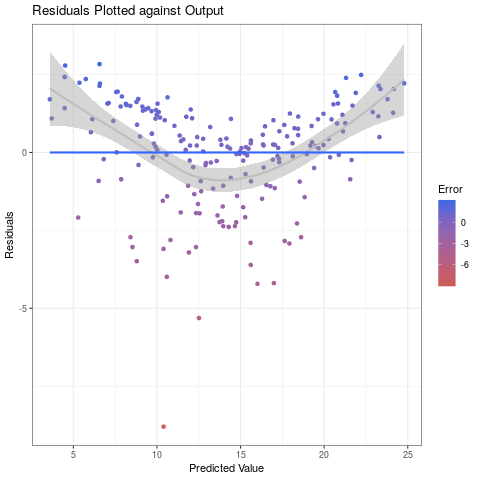
\includegraphics[width=.9\linewidth]{ResidualPlotMultLinRegIntroDataSci.png}
\end{center}

\begin{verbatim}
## `geom_smooth()` using method = 'loess' and formula 'y ~ x'
\end{verbatim}

\begin{center}
\includegraphics[width=.9\linewidth]{./attachments/MultLinReg727unnamed-chunk-14-1.png}
\end{center}

\item base
\label{sec:org16d78cc}
\begin{minted}[]{r}
plot(Error ~ Output, data = ResDF, pch = 19, col = "IndianRed", main = "Residuals against Predictions")
smooth <- loess(formula = Error ~ Output, data = ResDF, span = 0.8)
predict(smooth) %>% lines(col = "Blue")
abline(lm(Error ~ Output, data = ResDF), col = "Purple")
\end{minted}

\begin{center}
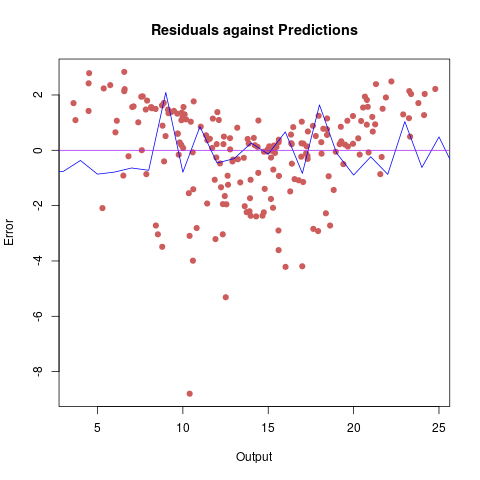
\includegraphics[width=.9\linewidth]{ResidualAgainstPredMultLinReg.png}
\end{center}

\begin{center}
\includegraphics[width=.9\linewidth]{./attachments/MultLinReg727unnamed-chunk-15-1.png}
\end{center}

\begin{HTML}
</div>
\end{HTML}

From this it can be seen that the residuals are centred around zero, but
they are not normally distributed, the model performance appears to fail
normality assumptions for values \(\in \left( 10, 20 \right)\)
\end{enumerate}

\subsubsection{(h) Plot the histogram of the residuals}
\label{sec:org196f8f2}
\begin{enumerate}
\item ggplot
\label{sec:orgcaf68ea}
\begin{enumerate}
\item Absolute Count
\label{sec:orgce7475e}
\begin{minted}[]{r}
ggplot(data = ResDF, aes(x = Error, col = Output)) +
  geom_histogram() +
  theme_classic() +
  labs(y = "Absolute Count", x = "Residual Value", title = "Residual Distribution") 
\end{minted}

\begin{center}
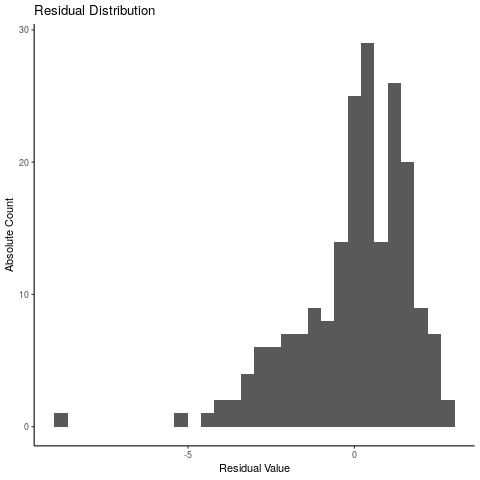
\includegraphics[width=.9\linewidth]{HistResGGMultLinReg.png}
\end{center}

\begin{verbatim}
## `stat_bin()` using `bins = 30`. Pick better value with `binwidth`.
\end{verbatim}

\begin{center}
\includegraphics[width=.9\linewidth]{./attachments/MultLinReg727unnamed-chunk-16-1.png}
\end{center}

\begin{minted}[]{elisp}
(setq org-complete-tags-always-offer-all-agenda-tags t)
(setq org-fast-tag-selection-single-key nil)
\end{minted}

\item Density\hfill{}\textsc{ggplot2:Histogram}
\label{sec:orge6d095e}
\begin{minted}[]{r}
df <- data.frame(x = rnorm(1000, 2, 2))

# overlay histogram and normal density
ggplot(ResDF, aes(x=Error)) +
  geom_histogram(aes(y = stat(density))) +
  stat_function(
    fun = dnorm, 
    args = list(mean = mean(df$x), sd = sd(df$x)), 
    lwd = 2, 
    col = 'IndianRed'
  ) +
  theme_classic() +
  labs(title = "Histogram of Residuals", y = "Density of Observations", x= "Residuals")
\end{minted}

\begin{center}
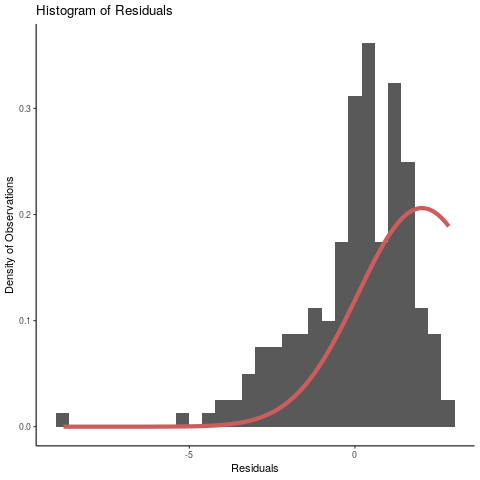
\includegraphics[width=.9\linewidth]{HistOverlayMultLinReg.png}
\end{center}

\begin{verbatim}
## `stat_bin()` using `bins = 30`. Pick better value with `binwidth`.
\end{verbatim}

\begin{center}
\includegraphics[width=.9\linewidth]{./attachments/MultLinReg727unnamed-chunk-17-1.png}
\end{center}

\item White Noise
\label{sec:orgcb26af2}
We can visualise the residuals as white noise:

\begin{enumerate}
\item Our Residuals
\label{sec:org855cc29}
\begin{minted}[]{r}
library(tidyverse)
## Put some White Noise on the ResDF
ResDF <- cbind(ResDF, "Wnoise" = rnorm(nrow(ResDF), mean = 0, sd = sd(ResDF$Error)))
head(ResDF)


## Our Residuals
ggplot(ResDF, aes(x = Input, y = Error, col = Output)) +
  geom_line() +
  geom_abline(slope = 0, intercept = 0, lty = "twodash", col = "IndianRed") +
  theme(legend.position = "none") + 
  labs(title = "Distribution of Residuals")
\end{minted}

\begin{center}
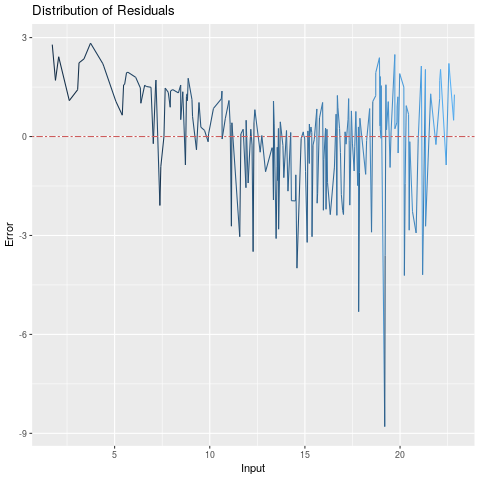
\includegraphics[width=.9\linewidth]{aljas.png}
\end{center}

\begin{center}
\includegraphics[width=.9\linewidth]{./attachments/MultLinReg727unnamed-chunk-18-1.png}
\end{center}

\begin{minted}[]{r}
## White Noise

ggplot(ResDF, aes(x = Input, y = Wnoise, col = Output)) +
  geom_line() +
  geom_abline(slope = 0, intercept = 0, lty = "twodash", col = "IndianRed") +
  theme(legend.position = "none") + 
  labs(title = "Distribution of Residuals")
\end{minted}

\begin{center}
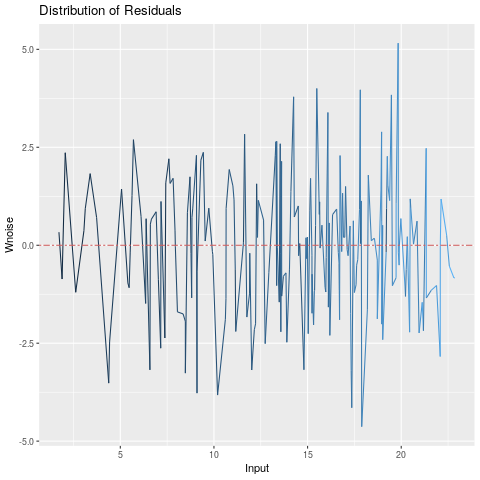
\includegraphics[width=.9\linewidth]{LinePlotResiduals.png}
\end{center}

\begin{center}
\includegraphics[width=.9\linewidth]{./attachments/MultLinReg727unnamed-chunk-18-2.png}
\end{center}

This clearly shows that the Residuals are non-normal.
\end{enumerate}
\end{enumerate}

\item Base\hfill{}\textsc{ggplot2:Histogram:BasePlot}
\label{sec:orgc927eab}
\begin{minted}[]{r}
hist(ResDF$Error
     , breaks = 30,
     prob=TRUE,
     lwd=2,
    main = "Residual Distribution",
    xlab = "Distance from the Model", border = "purple"
    ) 

  # Overlay the Normal Dist Curve
x <- 1:100    # Stupid base package wants some f(x), this is hacky but easier than stuffing around with lines or defining a function
curve(dnorm(x, mean(ResDF$Error), sd(ResDF$Error)), add=TRUE, col="purple", lwd=2) # Draws the actual density function

# lines(density(possibleyvals_conf), col='purple', lwd=2) # Draws the observed density function
lwr_conf <- qnorm(p = 0.05, mean(ResDF$Error), sd(ResDF$Error))
upr_conf <- qnorm(p = 1-0.05, mean(ResDF$Error), sd(ResDF$Error))
abline(v=upr_conf, col='pink', lwd=3)  
abline(v=lwr_conf, col='pink', lwd=3)     
abline(v=mean(ResDF$Error), lwd=2, lty='dotted')  
\end{minted}

\begin{center}
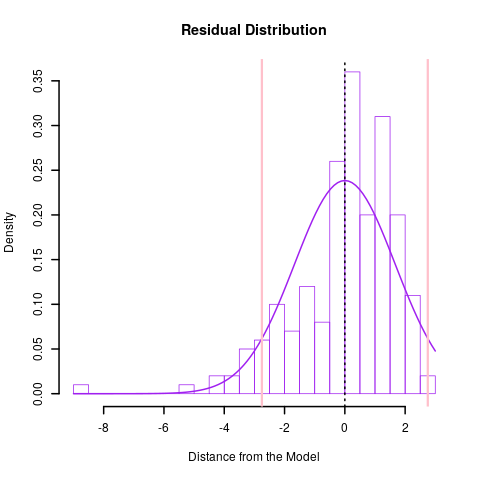
\includegraphics[width=.9\linewidth]{BasePlotResidualHistMultLinReg.png}
\end{center}

\begin{center}
\includegraphics[width=.9\linewidth]{./attachments/MultLinReg727unnamed-chunk-19-1.png}
\end{center}

\begin{minted}[]{r}
lwr_conf <- qnorm(p = 0.05, mean(ResDF$Error), sd(ResDF$Error))
upr_conf <- qnorm(p = 1-0.05, mean(ResDF$Error), sd(ResDF$Error))
\end{minted}

\begin{HTML}
</div>
\end{HTML}

It hence appears that the Residuals skewed left, which suggests an upper
bound on the residual value, the histogram is sufficiently non-normal to
reject the assumption that the residuals are normally distributed
\end{enumerate}

\subsubsection{(i) Comment on the residual plots}
\label{sec:orga06e321}
The Residuals can be analised by plotting the model:

\begin{minted}[]{r}
layout(matrix(data = 1:4, nrow = 2))
plot(advModMultb1)
\end{minted}

\begin{center}
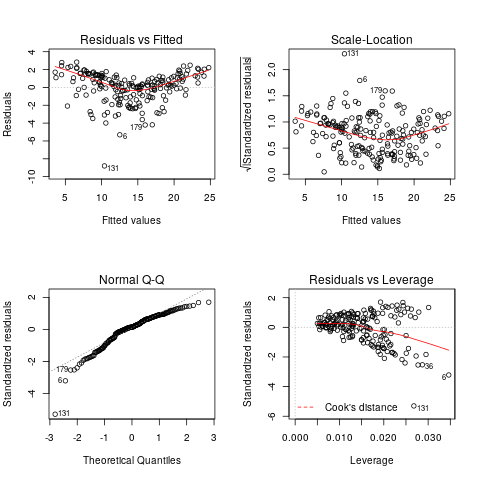
\includegraphics[width=.9\linewidth]{ResidualLinePlotMultLinReg.png}
\end{center}

\begin{center}
\includegraphics[width=.9\linewidth]{./attachments/MultLinReg727unnamed-chunk-21-1.png}
\end{center}\begin{center}
\includegraphics[width=.9\linewidth]{./attachments/MultLinReg727unnamed-chunk-21-2.png}
\end{center}\begin{center}
\includegraphics[width=.9\linewidth]{./attachments/MultLinReg727unnamed-chunk-21-3.png}
\end{center}\begin{center}
\includegraphics[width=.9\linewidth]{./attachments/MultLinReg727unnamed-chunk-21-4.png}
\end{center}

This is an inappropriate model because the residuals are non-normally
distributed.

\subsubsection{(j) Use the multivariate model for predictions}
\label{sec:org1afd5bd}
\begin{minted}[]{r}
newdata =  data.frame("TV" = c(3, 1, 2), "Radio" = c(4, 5, 6))
Mod_Adv_Mult_b1 <- predict(object = advModMultb1, newdata)

mypreds <- data.frame("Input" = newdata, "Output" =  Mod_Adv_Mult_b1)
mypreds # Careful with the names, they workout as Input.name in this case.
\end{minted}

\begin{verbatim}
##   Input.TV Input.Radio   Output
## 1        3           4 3.810341
## 2        1           5 3.906826
## 3        2           6 4.140575
\end{verbatim}

\subsection{Question 02: Non Linear Models: Use Advertising data set}
\label{sec:org1581a7b}
\subsubsection{(a) Add the Interaction Term TV*Radio and test the significance of}
\label{sec:org7fd3f26}
the interaction term \{.tabset\}
:CUSTOM\textsubscript{ID}: a-add-the-interaction-term-tvradio-and-test-the-significance-of-the-interaction-term-.tabset

reconsider the correlationplots:

\begin{enumerate}
\item Base
\label{sec:orga8baa5a}
\begin{minted}[]{r}
pairs(x = adv)
\end{minted}

\begin{center}
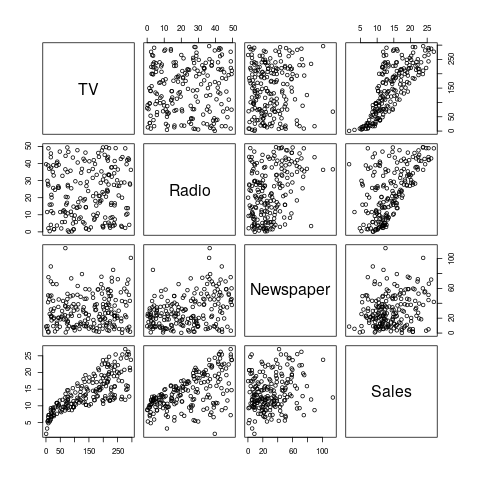
\includegraphics[width=.9\linewidth]{ResPlotAdvertisingMultLinReg2.png}
\end{center}

\begin{center}
\includegraphics[width=.9\linewidth]{./attachments/MultLinReg727unnamed-chunk-23-1.png}
\end{center}
\end{enumerate}

\subsubsection{corrplot}
\label{sec:orgdcff267}
\begin{minted}[]{r}
adv[, names(adv)!="Newspaper"] %>% cor() %>% corrplot(method = "ellipse", type = "lower")
\end{minted}

\begin{center}
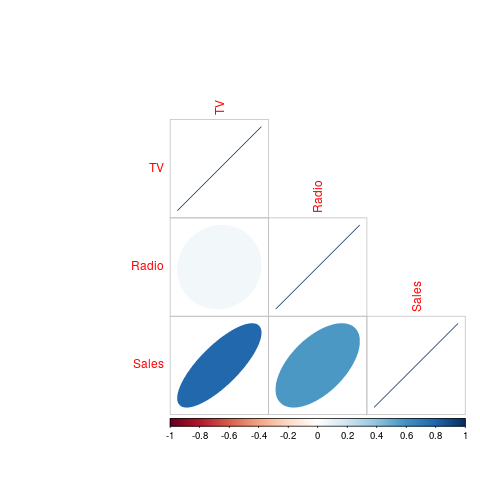
\includegraphics[width=.9\linewidth]{CorrelationPlotMultLinReg2.png}
\end{center}

\begin{center}
\includegraphics[width=.9\linewidth]{./attachments/MultLinReg727unnamed-chunk-24-1.png}
\end{center}

\begin{HTML}
</div>
\end{HTML}

From this we can determine that there is no interaction between TV and
radio (however previously there was interaction between newspaper and
Radio, we should consider that next)

\begin{enumerate}
\item Create the MLReg
\label{sec:orga31d01d}
\begin{minted}[]{r}
int_mod_adv <- lm(formula = Sales ~ TV * Radio + TV + Radio, data = adv)
int_mod_adv
\end{minted}

\begin{verbatim}
## 
## Call:
## lm(formula = Sales ~ TV * Radio + TV + Radio, data = adv)
## 
## Coefficients:
## (Intercept)           TV        Radio     TV:Radio  
##    6.750220     0.019101     0.028860     0.001086
\end{verbatim}

\begin{minted}[]{r}
summary(int_mod_adv)
\end{minted}

\begin{verbatim}
## 
## Call:
## lm(formula = Sales ~ TV * Radio + TV + Radio, data = adv)
## 
## Residuals:
##     Min      1Q  Median      3Q     Max 
## -6.3366 -0.4028  0.1831  0.5948  1.5246 
## 
## Coefficients:
##              Estimate Std. Error t value Pr(>|t|)    
## (Intercept) 6.750e+00  2.479e-01  27.233   <2e-16 ***
## TV          1.910e-02  1.504e-03  12.699   <2e-16 ***
## Radio       2.886e-02  8.905e-03   3.241   0.0014 ** 
## TV:Radio    1.086e-03  5.242e-05  20.727   <2e-16 ***
## ---
## Signif. codes:  0 '***' 0.001 '**' 0.01 '*' 0.05 '.' 0.1 ' ' 1
## 
## Residual standard error: 0.9435 on 196 degrees of freedom
## Multiple R-squared:  0.9678, Adjusted R-squared:  0.9673 
## F-statistic:  1963 on 3 and 196 DF,  p-value: < 2.2e-16
\end{verbatim}
\end{enumerate}

\subsubsection{(b) Give the resulting model after considering this interaction}
\label{sec:org46b2268}
term.
:CUSTOM\textsubscript{ID}: b-give-the-resulting-model-after-considering-this-interaction-term.

The model will be of the form:

$$
  \text{Sales} = 0.0019 \times \text{TV} \times + \text{Radio} \times  0.002886 + \text{TV} \times \text{Radio} \times 0.001086
  $$

Note that all the terms of the model are significant, hence we deem the
model as adequate.

\subsubsection{(c) Construct the Polynomial Regression Model of order 3 and test}
\label{sec:orgda1638b}
the model significance
:CUSTOM\textsubscript{ID}: c-construct-the-polynomial-regression-model-of-order-3-and-test-the-model-significance

When creating polynomial models there are raw and orthogonal
polynomials,

\begin{itemize}
\item A raw polynomial will be the the standard System of equations that you
get by minimising the RSS

\begin{itemize}
\item The problem with this is that the values will be correlated with
each other
\end{itemize}

\item An orthogonal polynomial is a transformed but equivalent polynomial

\begin{itemize}
\item The advantage to this is that the p-value's will be moremeaningful
because the coefficients aren't correlated with each other
\item The disadvantage is that the values are not directly related to our
data and are not hence meaningful.
\end{itemize}
\end{itemize}

\begin{minted}[]{r}
# Orthogonal (fixes the correlation between the coefficients))

polymodel_Orth <- lm(Sales ~ poly(x = TV, degree = 3, raw = FALSE), data = adv)
summary(polymodel_Orth)
\end{minted}

\begin{verbatim}
## 
## Call:
## lm(formula = Sales ~ poly(x = TV, degree = 3, raw = FALSE), data = adv)
## 
## Residuals:
##     Min      1Q  Median      3Q     Max 
## -7.9734 -1.8900 -0.0897  2.0189  7.3765 
## 
## Coefficients:
##                                        Estimate Std. Error t value
## (Intercept)                             14.0225     0.2286  61.353
## poly(x = TV, degree = 3, raw = FALSE)1  57.5727     3.2322  17.812
## poly(x = TV, degree = 3, raw = FALSE)2  -6.2288     3.2322  -1.927
## poly(x = TV, degree = 3, raw = FALSE)3   4.0074     3.2322   1.240
##                                        Pr(>|t|)    
## (Intercept)                              <2e-16 ***
## poly(x = TV, degree = 3, raw = FALSE)1   <2e-16 ***
## poly(x = TV, degree = 3, raw = FALSE)2   0.0554 .  
## poly(x = TV, degree = 3, raw = FALSE)3   0.2165    
## ---
## Signif. codes:  0 '***' 0.001 '**' 0.01 '*' 0.05 '.' 0.1 ' ' 1
## 
## Residual standard error: 3.232 on 196 degrees of freedom
## Multiple R-squared:  0.622,  Adjusted R-squared:  0.6162 
## F-statistic: 107.5 on 3 and 196 DF,  p-value: < 2.2e-16
\end{verbatim}

\begin{minted}[]{r}
# Pure/Raw (has the advantage that you can interpret the coefficients, but the coefficients will depend on each other and be hence correlated.)

polymodel <- lm(Sales ~ I(TV*TV*TV) + I(TV*TV) + (TV), data = adv)
summary(polymodel)    # I is used to inhibit the interpretation of * as relating to the model,
\end{minted}

\begin{verbatim}
## 
## Call:
## lm(formula = Sales ~ I(TV * TV * TV) + I(TV * TV) + (TV), data = adv)
## 
## Residuals:
##     Min      1Q  Median      3Q     Max 
## -7.9734 -1.8900 -0.0897  2.0189  7.3765 
## 
## Coefficients:
##                   Estimate Std. Error t value Pr(>|t|)    
## (Intercept)      5.420e+00  8.641e-01   6.272 2.23e-09 ***
## I(TV * TV * TV)  5.572e-07  4.494e-07   1.240 0.216519    
## I(TV * TV)      -3.152e-04  2.022e-04  -1.559 0.120559    
## TV               9.643e-02  2.580e-02   3.738 0.000243 ***
## ---
## Signif. codes:  0 '***' 0.001 '**' 0.01 '*' 0.05 '.' 0.1 ' ' 1
## 
## Residual standard error: 3.232 on 196 degrees of freedom
## Multiple R-squared:  0.622,  Adjusted R-squared:  0.6162 
## F-statistic: 107.5 on 3 and 196 DF,  p-value: < 2.2e-16
\end{verbatim}

\begin{minted}[]{r}
                            # Instead of representing interaction it represents TV^3

polymodel_Raw<- lm(Sales ~ poly(x = TV, degree = 3, raw = TRUE), data = adv)
summary(polymodel_Raw)
\end{minted}

\begin{verbatim}
## 
## Call:
## lm(formula = Sales ~ poly(x = TV, degree = 3, raw = TRUE), data = adv)
## 
## Residuals:
##     Min      1Q  Median      3Q     Max 
## -7.9734 -1.8900 -0.0897  2.0189  7.3765 
## 
## Coefficients:
##                                         Estimate Std. Error t value
## (Intercept)                            5.420e+00  8.641e-01   6.272
## poly(x = TV, degree = 3, raw = TRUE)1  9.643e-02  2.580e-02   3.738
## poly(x = TV, degree = 3, raw = TRUE)2 -3.152e-04  2.022e-04  -1.559
## poly(x = TV, degree = 3, raw = TRUE)3  5.572e-07  4.494e-07   1.240
##                                       Pr(>|t|)    
## (Intercept)                           2.23e-09 ***
## poly(x = TV, degree = 3, raw = TRUE)1 0.000243 ***
## poly(x = TV, degree = 3, raw = TRUE)2 0.120559    
## poly(x = TV, degree = 3, raw = TRUE)3 0.216519    
## ---
## Signif. codes:  0 '***' 0.001 '**' 0.01 '*' 0.05 '.' 0.1 ' ' 1
## 
## Residual standard error: 3.232 on 196 degrees of freedom
## Multiple R-squared:  0.622,  Adjusted R-squared:  0.6162 
## F-statistic: 107.5 on 3 and 196 DF,  p-value: < 2.2e-16
\end{verbatim}

The 3rd degree coefficient is not significant, hence we consider the 2nd
degree:

\begin{minted}[]{r}
quadmod <- lm(formula = Sales ~ I(TV*TV) + TV, data = adv)
summary(quadmod)
\end{minted}

\begin{verbatim}
## 
## Call:
## lm(formula = Sales ~ I(TV * TV) + TV, data = adv)
## 
## Residuals:
##     Min      1Q  Median      3Q     Max 
## -7.6844 -1.7843 -0.1562  2.0088  7.5097 
## 
## Coefficients:
##               Estimate Std. Error t value Pr(>|t|)    
## (Intercept)  6.114e+00  6.592e-01   9.275  < 2e-16 ***
## I(TV * TV)  -6.847e-05  3.558e-05  -1.924   0.0557 .  
## TV           6.727e-02  1.059e-02   6.349 1.46e-09 ***
## ---
## Signif. codes:  0 '***' 0.001 '**' 0.01 '*' 0.05 '.' 0.1 ' ' 1
## 
## Residual standard error: 3.237 on 197 degrees of freedom
## Multiple R-squared:  0.619,  Adjusted R-squared:  0.6152 
## F-statistic: 160.1 on 2 and 197 DF,  p-value: < 2.2e-16
\end{verbatim}

The quadratic term is not sufficiently significant so the model is
rejected

\subsubsection{(d) Give the resulting selected model}
\label{sec:org1bd734f}
The model selected is the multiple linear regression with the
interaction from before:

$$
  \text{Sales} = 0.0019 \times \text{TV} \times + \text{Radio} \times  0.002886 + \text{TV} \times \text{Radio} \times 0.001086
  $$

This was converted from `md` to `org` using `pandoc -f gfm` at time: 
2020-02-08T05-00-13
\end{document}